% Options for packages loaded elsewhere
\PassOptionsToPackage{unicode}{hyperref}
\PassOptionsToPackage{hyphens}{url}
%
\documentclass[
  ignorenonframetext,
]{beamer}
\usepackage{pgfpages}
\setbeamertemplate{caption}[numbered]
\setbeamertemplate{caption label separator}{: }
\setbeamercolor{caption name}{fg=normal text.fg}
\beamertemplatenavigationsymbolsempty
% Prevent slide breaks in the middle of a paragraph
\widowpenalties 1 10000
\raggedbottom
\setbeamertemplate{part page}{
  \centering
  \begin{beamercolorbox}[sep=16pt,center]{part title}
    \usebeamerfont{part title}\insertpart\par
  \end{beamercolorbox}
}
\setbeamertemplate{section page}{
  \centering
  \begin{beamercolorbox}[sep=12pt,center]{part title}
    \usebeamerfont{section title}\insertsection\par
  \end{beamercolorbox}
}
\setbeamertemplate{subsection page}{
  \centering
  \begin{beamercolorbox}[sep=8pt,center]{part title}
    \usebeamerfont{subsection title}\insertsubsection\par
  \end{beamercolorbox}
}
\AtBeginPart{
  \frame{\partpage}
}
\AtBeginSection{
  \ifbibliography
  \else
    \frame{\sectionpage}
  \fi
}
\AtBeginSubsection{
  \frame{\subsectionpage}
}

\usepackage{amsmath,amssymb}
\usepackage{lmodern}
\usepackage{iftex}
\ifPDFTeX
  \usepackage[T1]{fontenc}
  \usepackage[utf8]{inputenc}
  \usepackage{textcomp} % provide euro and other symbols
\else % if luatex or xetex
  \usepackage{unicode-math}
  \defaultfontfeatures{Scale=MatchLowercase}
  \defaultfontfeatures[\rmfamily]{Ligatures=TeX,Scale=1}
\fi
% Use upquote if available, for straight quotes in verbatim environments
\IfFileExists{upquote.sty}{\usepackage{upquote}}{}
\IfFileExists{microtype.sty}{% use microtype if available
  \usepackage[]{microtype}
  \UseMicrotypeSet[protrusion]{basicmath} % disable protrusion for tt fonts
}{}
\makeatletter
\@ifundefined{KOMAClassName}{% if non-KOMA class
  \IfFileExists{parskip.sty}{%
    \usepackage{parskip}
  }{% else
    \setlength{\parindent}{0pt}
    \setlength{\parskip}{6pt plus 2pt minus 1pt}}
}{% if KOMA class
  \KOMAoptions{parskip=half}}
\makeatother
\usepackage{xcolor}
\newif\ifbibliography
\setlength{\emergencystretch}{3em} % prevent overfull lines
\setcounter{secnumdepth}{-\maxdimen} % remove section numbering


\providecommand{\tightlist}{%
  \setlength{\itemsep}{0pt}\setlength{\parskip}{0pt}}\usepackage{longtable,booktabs,array}
\usepackage{calc} % for calculating minipage widths
\usepackage{caption}
% Make caption package work with longtable
\makeatletter
\def\fnum@table{\tablename~\thetable}
\makeatother
\usepackage{graphicx}
\makeatletter
\def\maxwidth{\ifdim\Gin@nat@width>\linewidth\linewidth\else\Gin@nat@width\fi}
\def\maxheight{\ifdim\Gin@nat@height>\textheight\textheight\else\Gin@nat@height\fi}
\makeatother
% Scale images if necessary, so that they will not overflow the page
% margins by default, and it is still possible to overwrite the defaults
% using explicit options in \includegraphics[width, height, ...]{}
\setkeys{Gin}{width=\maxwidth,height=\maxheight,keepaspectratio}
% Set default figure placement to htbp
\makeatletter
\def\fps@figure{htbp}
\makeatother

\makeatletter
\@ifpackageloaded{tcolorbox}{}{\usepackage[many]{tcolorbox}}
\@ifpackageloaded{fontawesome5}{}{\usepackage{fontawesome5}}
\definecolor{quarto-callout-color}{HTML}{909090}
\definecolor{quarto-callout-note-color}{HTML}{0758E5}
\definecolor{quarto-callout-important-color}{HTML}{CC1914}
\definecolor{quarto-callout-warning-color}{HTML}{EB9113}
\definecolor{quarto-callout-tip-color}{HTML}{00A047}
\definecolor{quarto-callout-caution-color}{HTML}{FC5300}
\definecolor{quarto-callout-color-frame}{HTML}{acacac}
\definecolor{quarto-callout-note-color-frame}{HTML}{4582ec}
\definecolor{quarto-callout-important-color-frame}{HTML}{d9534f}
\definecolor{quarto-callout-warning-color-frame}{HTML}{f0ad4e}
\definecolor{quarto-callout-tip-color-frame}{HTML}{02b875}
\definecolor{quarto-callout-caution-color-frame}{HTML}{fd7e14}
\makeatother
\makeatletter
\makeatother
\makeatletter
\makeatother
\makeatletter
\@ifpackageloaded{caption}{}{\usepackage{caption}}
\AtBeginDocument{%
\ifdefined\contentsname
  \renewcommand*\contentsname{Table of contents}
\else
  \newcommand\contentsname{Table of contents}
\fi
\ifdefined\listfigurename
  \renewcommand*\listfigurename{List of Figures}
\else
  \newcommand\listfigurename{List of Figures}
\fi
\ifdefined\listtablename
  \renewcommand*\listtablename{List of Tables}
\else
  \newcommand\listtablename{List of Tables}
\fi
\ifdefined\figurename
  \renewcommand*\figurename{Figure}
\else
  \newcommand\figurename{Figure}
\fi
\ifdefined\tablename
  \renewcommand*\tablename{Table}
\else
  \newcommand\tablename{Table}
\fi
}
\@ifpackageloaded{float}{}{\usepackage{float}}
\floatstyle{ruled}
\@ifundefined{c@chapter}{\newfloat{codelisting}{h}{lop}}{\newfloat{codelisting}{h}{lop}[chapter]}
\floatname{codelisting}{Listing}
\newcommand*\listoflistings{\listof{codelisting}{List of Listings}}
\makeatother
\makeatletter
\@ifpackageloaded{caption}{}{\usepackage{caption}}
\@ifpackageloaded{subcaption}{}{\usepackage{subcaption}}
\makeatother
\makeatletter
\@ifpackageloaded{tcolorbox}{}{\usepackage[many]{tcolorbox}}
\makeatother
\makeatletter
\@ifundefined{shadecolor}{\definecolor{shadecolor}{rgb}{.97, .97, .97}}
\makeatother
\makeatletter
\makeatother
\ifLuaTeX
  \usepackage{selnolig}  % disable illegal ligatures
\fi
\IfFileExists{bookmark.sty}{\usepackage{bookmark}}{\usepackage{hyperref}}
\IfFileExists{xurl.sty}{\usepackage{xurl}}{} % add URL line breaks if available
\urlstyle{same} % disable monospaced font for URLs
\hypersetup{
  pdftitle={Chapter 9},
  pdfauthor={Holly Steeves},
  hidelinks,
  pdfcreator={LaTeX via pandoc}}

\title{Chapter 9}
\author{Holly Steeves}
\date{}

\begin{document}
\frame{\titlepage}
\ifdefined\Shaded\renewenvironment{Shaded}{\begin{tcolorbox}[interior hidden, enhanced, sharp corners, borderline west={3pt}{0pt}{shadecolor}, breakable, frame hidden, boxrule=0pt]}{\end{tcolorbox}}\fi

\hypertarget{hypotheses-and-test-procedures}{%
\section{9.1 Hypotheses and Test
Procedures}\label{hypotheses-and-test-procedures}}

\begin{frame}{Outcomes}
\protect\hypertarget{outcomes}{}
By the end of this section, you will be able to:

\begin{itemize}[<+->]
\tightlist
\item
  Define, identify, or determine the null and alternate hypotheses of a
  given problem.
\item
  Define, identify and use the test statistic and rejection region of a
  given test procedure.
\item
  Write what a type I error or a type II error mean in the context of a
  given test of hypotheses.
\item
  Determine the probabilities of type I and type II errors.
\end{itemize}
\end{frame}

\begin{frame}{Introduction}
\protect\hypertarget{introduction}{}
\begin{itemize}[<+->]
\tightlist
\item
  A parameter can be estimated from sample data either by a single
  number (a point estimate) or an entire interval of plausible values (a
  confidence interval).
\item
  Frequently, however, the objective of an investigation is not to
  estimate a parameter but to decide which of two contradictory claims
  about the parameter is correct.
\item
  Methods for accomplishing this are the part of inference called
  \textbf{hypothesis testing}.
\item
  In this chapter, we first discuss some of the basic concepts and
  terminology in hypothesis testing and then develop decision procedures
  for the most frequently encountered testing problems based on a sample
  from a single population.
\end{itemize}
\end{frame}

\begin{frame}{Hypotheses}
\protect\hypertarget{hypotheses}{}
\begin{tcolorbox}[enhanced jigsaw, left=2mm, breakable, bottomrule=.15mm, colframe=quarto-callout-important-color-frame, arc=.35mm, leftrule=.75mm, colbacktitle=quarto-callout-important-color!10!white, titlerule=0mm, opacityback=0, coltitle=black, opacitybacktitle=0.6, colback=white, toprule=.15mm, toptitle=1mm, bottomtitle=1mm, title=\textcolor{quarto-callout-important-color}{\faExclamation}\hspace{0.5em}{Definition}, rightrule=.15mm]

A \textbf{statistical hypotheses} is a claim either about the value of a
single parameter, about the values of several parameters, or about the
form of an entire probability distribution.

\end{tcolorbox}
\end{frame}

\begin{frame}{Hypotheses}
\protect\hypertarget{hypotheses-1}{}
Examples:

\begin{itemize}[<+->]
\tightlist
\item
  \(\mu = 311\), where \(\mu\) is the true average one--term textbook
  expenditure for students at a university.
\item
  \(p < 0.50\), where \(p\) is the proportion of adults who approve of
  the job that the President is doing.
\item
  If \(\mu_{1}\) and \(\mu_{2}\) denote the true average decreases in
  systolic blood pressure for two different drugs, one hypothesis is the
  assertion that \(\mu_{1} - \mu_{2} = 0\), and another is the statement
  \(\mu_{1} - \mu_{2} > 5\).
\item
  Yet another example of a hypothesis is that the stopping distance for
  a car under particular conditions has a normal distribution.
\end{itemize}
\end{frame}

\begin{frame}{Null Hypothesis}
\protect\hypertarget{null-hypothesis}{}
\begin{tcolorbox}[enhanced jigsaw, left=2mm, breakable, bottomrule=.15mm, colframe=quarto-callout-important-color-frame, arc=.35mm, leftrule=.75mm, colbacktitle=quarto-callout-important-color!10!white, titlerule=0mm, opacityback=0, coltitle=black, opacitybacktitle=0.6, colback=white, toprule=.15mm, toptitle=1mm, bottomtitle=1mm, title=\textcolor{quarto-callout-important-color}{\faExclamation}\hspace{0.5em}{Definition}, rightrule=.15mm]

The \textbf{null hypothesis}, denoted by \(H_{0}\), is the claim that is
initially assumed to be true (the ``prior belief'' claim). The
alternative hypothesis, denoted by \(H_{a}\), is the assertion that is
contradictory to \(H_{0}\).

The null hypothesis will be rejected in favor of the alternative
hypothesis only if sample evidence suggests that \(H_{0}\) is false. If
the sample does not strongly contradict \(H_{0}\), we will continue to
believe in the plausibility of the null hypothesis. The two possible
conclusions from a hypothesis

\begin{itemize}[<+->]
\tightlist
\item
  reject \(H_{0}\)
\item
  fail to reject \(H_{0}\).
\end{itemize}

\end{tcolorbox}
\end{frame}

\begin{frame}{Tests of Hypotheses}
\protect\hypertarget{tests-of-hypotheses}{}
\begin{tcolorbox}[enhanced jigsaw, left=2mm, breakable, bottomrule=.15mm, colframe=quarto-callout-important-color-frame, arc=.35mm, leftrule=.75mm, colbacktitle=quarto-callout-important-color!10!white, titlerule=0mm, opacityback=0, coltitle=black, opacitybacktitle=0.6, colback=white, toprule=.15mm, toptitle=1mm, bottomtitle=1mm, title=\textcolor{quarto-callout-important-color}{\faExclamation}\hspace{0.5em}{Definition}, rightrule=.15mm]

A \textbf{test of hypotheses} is a method for using sample data to
decide whether the null hypothesis should be rejected.

Ex: Test \(H_{0}: \mu = 750\) versus \(H_{a}: \mu \neq 750\).

Only if the sample data suggests that \(\mu\) is something other than
750 should the null hypothesis be rejected for the alternative
hypothesis.

\end{tcolorbox}
\end{frame}

\begin{frame}{Tests of Hypothesis}
\protect\hypertarget{tests-of-hypothesis}{}
The alternative to \(H_{0}: \theta = \theta_{0}\) will be one of the
following:

\begin{enumerate}[<+->]
\tightlist
\item
  \(H_{a}: \theta < \theta_{0}\).
\item
  \(H_{a}: \theta > \theta_{0}\).
\item
  \(H_{a}: \theta \neq \theta_{0}\).
\end{enumerate}

where \(\theta_{0}\) is called the \emph{null value}.
\end{frame}

\begin{frame}{Test Procedures}
\protect\hypertarget{test-procedures}{}
\begin{itemize}[<+->]
\tightlist
\item
  A \textbf{test procedure} is a rule, based on sample data, for
  deciding whether or not to reject \(H_{0}\) for \(H_{a}\).
\end{itemize}

\begin{tcolorbox}[enhanced jigsaw, left=2mm, breakable, bottomrule=.15mm, colframe=quarto-callout-important-color-frame, arc=.35mm, leftrule=.75mm, colbacktitle=quarto-callout-important-color!10!white, titlerule=0mm, opacityback=0, coltitle=black, opacitybacktitle=0.6, colback=white, toprule=.15mm, toptitle=1mm, bottomtitle=1mm, title=\textcolor{quarto-callout-important-color}{\faExclamation}\hspace{0.5em}{Test Procedure}, rightrule=.15mm]

A test procedure is specified by the following:

\begin{enumerate}[<+->]
\tightlist
\item
  A \textbf{test statistic}, which is a function of the sample data on
  which the decision is based.
\item
  A \textbf{rejection region}, which is the set of all test statistic
  values for which \(H_{0}\) will be rejected.
\end{enumerate}

The null hypothesis will be rejected if and only if the observed test
statistic falls in the rejection region.

\end{tcolorbox}
\end{frame}

\begin{frame}{Example}
\protect\hypertarget{example}{}
Suppose a cigarette manufacturer claims that the average nicotine
content \(\mu\) of brand B cigarettes is (at most) 1.5 mg. It would be
unwise to reject the manufacturer's claim without strong contradictory
evidence, so an appropriate problem formulation is to test
\(H_{0}: \mu = 1.5\) versus \(H_{a}: \mu > 1.5\).

Consider a decision rule based on analyzing a random sample of 32
cigarettes. Let \(\bar{X}\) denote the sample average nicotine content.
If \(H_{0}\) is true, \(E[\bar{X}] = \mu = 1.5\), whereas if \(H_{0}\)
is false, we expect \(\bar{X}\) to exceed 1.5.

Strong evidence against \(H_{0}\) is provided by a value \(\bar{x}\)
that considerably exceeds 1.5. Thus we might use \(\bar{X}\) as a test
statistic along with the rejection region \(\bar{x} > 1.60\).
\end{frame}

\begin{frame}{Errors in Testing}
\protect\hypertarget{errors-in-testing}{}
\begin{itemize}[<+->]
\tightlist
\item
  We make a decision about the parameter, but what if we make the wrong
  decision?
\item
  We won't always be right! So let's consider the types of errors that
  we could make.
\end{itemize}

\begin{tcolorbox}[enhanced jigsaw, left=2mm, breakable, bottomrule=.15mm, colframe=quarto-callout-important-color-frame, arc=.35mm, leftrule=.75mm, colbacktitle=quarto-callout-important-color!10!white, titlerule=0mm, opacityback=0, coltitle=black, opacitybacktitle=0.6, colback=white, toprule=.15mm, toptitle=1mm, bottomtitle=1mm, title=\textcolor{quarto-callout-important-color}{\faExclamation}\hspace{0.5em}{Errors}, rightrule=.15mm]

\textbf{Type I Error}: Reject \(H_{0}\) when \(H_{0}\) is true.

\textbf{Type II Error}: Fail to reject \(H_{0}\) when \(H_{a}\) is true.

\end{tcolorbox}

\begin{longtable}[]{@{}lll@{}}
\toprule()
& \(H_{a}\) true & \(H_{0}\) true \\
\midrule()
\endhead
Reject \(H_{0}\) & :) & Type I \\
Fail to reject \(H_{0}\) & Type II & :) \\
\bottomrule()
\end{longtable}
\end{frame}

\begin{frame}{Example}
\protect\hypertarget{example-1}{}
In the nicotine scenario:

\textbf{Type I error} - rejecting \(H_{0}: \mu = 1.5\) for
\(H_{a}: \mu > 1.5\), when in fact \(\mu \ngtr 1.5\). That is, we
concluded that the mean nicotine content of brand B cigarettes is
greater than 1.5mg when in fact it isn't.

\textbf{Type II error} - failing to reject \(H_{0}: \mu = 1.5\) for
\(H_{a}: \mu > 1.5\) when in fact it is. That is, we failed to conclude
that the mean nicotine content of brand B cigarettes is greater than
1.5mg when in fact it is.
\end{frame}

\begin{frame}{Exercise 8}
\protect\hypertarget{exercise-8}{}
A regular type of laminate is currently being used by a manufacturer of
circuit boards. A special laminate has been developed to reduce warpage.
The regular laminate will be used on one sample of specimens and the
special laminate on another sample, and the amount of warpage will then
be determined for each specimen. The manufacturer will then switch to
the special laminate only if it can be demonstrated that the true
average amount of warpage for that laminate is less than for the regular
laminate. State the relevant hypotheses, and describe the type I and
type II errors in the context of this situation.
\end{frame}

\begin{frame}{Error Probabilities}
\protect\hypertarget{error-probabilities}{}
\begin{itemize}[<+->]
\tightlist
\item
  We cannot ever be 100\% sure that our decision was correct, therefore
  we always have the potential to make an error.
\item
  We must look for procedures for which either type of error is unlikely
  to occur. That is, a good procedure is one for which the probability
  of making either type of error is small.
\item
  The choice of a particular rejection region cutoff value fixes the
  probabilities of type I and type II errors. These error probabilities
  are traditionally denoted by \(\alpha\) and \(\beta\), respectively.
\item
  Because \(H_{0}\) specifies a unique value of the parameter, there is
  a single value of \(\alpha\). However, there is a different value of
  \(\beta\) for each value of the parameter consistent with \(H_{a}\).
\end{itemize}
\end{frame}

\begin{frame}{Example}
\protect\hypertarget{example-2}{}
An automobile model is known to sustain no visible damage 25\% of the
time in 10-mph crash tests. A modified bumper design has been proposed
in an effort to increase this percentage. Let \(p\) denote the
proportion of all 10-mph crashes with this new bumper that result in no
visible damage. The hypotheses to be tested are:

\[
H_{0}: p = 0.25
\]

(no improvement)

\[
H_{a}: p > 0.25
\]
\end{frame}

\begin{frame}{Example}
\protect\hypertarget{example-3}{}
The test will be based on an experiment involving \(n=20\) independent
crashes with prototypes of the new design. Intuitively, \(H_{0}\) should
be rejected if a substantial number of the crashes show no damage.
Consider the following test procedure:

Test Statistic: X = the number of crashes with no visible damage\\
Rejection region: \(R = \{8, 9, 10, ..., 19, 20 \}\); that is, reject
\(H_{0}\) if \(x \geq 8\), where \(x\) is the observed value of the test
statistic.

This rejection region is called \emph{upper-tailed} because it consists
only of large values of the test statistic.
\end{frame}

\begin{frame}{Example}
\protect\hypertarget{example-4}{}
When \(H_{0}\) is true, \(X\) has a binomial probability distribution
with \(n=20\) and \(p=0.25\). Then:

\[
\begin{aligned}
\alpha &= P(\text{type I error}) \\
&= P(H_{0} \text{ is rejected when it is true}) \\
&= P(X \geq 8 \text{ when } X \sim Bin(20,0.25)) \\
&= 1 - B(7; 20, 0.25)\\
&= 1 - 0.898 \\
&= 0.102 
\end{aligned}
\]

That is, when \(H_{0}\) is actually true, roughly 10\% of all
experiments consisting of 20 crashes would result in \(H_{0}\) being
incorrectly rejected (a type I error).
\end{frame}

\begin{frame}{Example}
\protect\hypertarget{example-5}{}
In contrast to \(\alpha\), there is not a single \(\beta\). Instead,
there is a different \(\beta\) for each different \(p\) that exceeds
0.25. Thus there is a value of \(\beta\) for \(p=0.3\), and another for
\(p=0.5\) and so on. For example:

\[
\begin{aligned}
\beta(0.3) &- P(\text{type II error when } p = 0.3) \\
&= P(H_{0} \text{ is not rejected when it is false because } p = 0.3) \\
&= P(X \leq 7 \text{ when } X \sim Bin(20, 0.30)) \\
&= B(7; 20, 0.3) \\
&= 0.772
\end{aligned}
\]

When \(p\) is actually 0.30, roughly 77\% of all experiments of this
type would result in \(H_{0}\) being incorrectly not rejected!
\end{frame}

\begin{frame}{Example}
\protect\hypertarget{example-6}{}
The proposed test procedure is still reasonable for testing the more
realistic null hypothesis that \(p \leq 0.25\). In this case, there is
no longer a single \(\alpha\), but instead there is an \(\alpha\) for
each \(p\) that is at most 0.25: \(\alpha(0.25)\), \(\alpha(0.23)\),
\(\alpha(0.20)\), \(\alpha(0.15)\), and so on. It is easily verified
that \(\alpha(p) < \alpha(0.25) = 0.102\) if \(p<0.25\). That is, the
largest value of \(\alpha\) occurs for the boundary value \(0.25\)
between \(H_{0}\) and \(H_{a}\). Thus, if \(\alpha\) is small for the
simplified null hypothesis, it will also be as small as or smaller for
the more realistic \(H_{0}\).
\end{frame}

\begin{frame}{Exercise 10}
\protect\hypertarget{exercise-10}{}
For healthy individuals the level of prothrombin in the blood is
approximately normally distributed with mean 20 mg/100 mL and standard
deviation 4 mg/100 mL. Low levels indicate low clotting ability. In
studying the effect of gallstones on prothrombin, the level of each
patient in a sample is measured to see if there is a deficiency. Let
\(\mu\) be the true average level of prothrombin for gallstone patients.

\begin{enumerate}[<+->]
[a.]
\tightlist
\item
  What are the appropriate null and alternative hypotheses?
\item
  Let \(\bar{X}\) denote the sample average level of prothrombin in a
  sample of \(n=20\) randomly selected gallstone patients. Consider the
  test procedure with test statistic \(\bar{X}\) and rejection region
  \(\bar{x} \leq 17.92\). What is the probability distribution of the
  test statistic when \(H_{0}\) is true? What is the probability of a
  type I error for the test procedure?
\end{enumerate}
\end{frame}

\begin{frame}{Exercise 10}
\protect\hypertarget{exercise-10-1}{}
\begin{enumerate}[<+->]
[a.]
\setcounter{enumi}{2}
\tightlist
\item
  What is the probability distribution of the test statistic when
  \(\mu = 16.7\)? Using the test procedure of part (b), what is the
  probability that gallstone patients will be judged not deficient in
  prothrombin, when in fact \(\mu = 16.7\) (a type II error).
\item
  How would you change the test procedure of part (b) to obtain a test
  with significance level 0.05? What impact would this change have on
  the error probability of part (c)?
\item
  Consider the standardized test statistic
  \(Z = (\bar{X} - 20)/(\sigma/\sqrt{n}) = (\bar{X} - 20)/0.8944\). What
  are the values of \(Z\) corresponding to the rejection region of part
  (b)?
\end{enumerate}
\end{frame}

\begin{frame}{Relationship between \(\alpha\) and \(\beta\)}
\protect\hypertarget{relationship-between-alpha-and-beta}{}
\begin{tcolorbox}[enhanced jigsaw, left=2mm, breakable, bottomrule=.15mm, colframe=quarto-callout-important-color-frame, arc=.35mm, leftrule=.75mm, colbacktitle=quarto-callout-important-color!10!white, titlerule=0mm, opacityback=0, coltitle=black, opacitybacktitle=0.6, colback=white, toprule=.15mm, toptitle=1mm, bottomtitle=1mm, title=\textcolor{quarto-callout-important-color}{\faExclamation}\hspace{0.5em}{Proposition}, rightrule=.15mm]

Suppose an experiment and a sample size are fixed and a test statistic
is chosen. Then decreasing the size of the rejection region to obtain a
smaller value of \(\alpha\) results in a larger value of \(\beta\) for
any particular parameter value consistent with \(H_{a}\).

\end{tcolorbox}
\end{frame}

\begin{frame}{Summary}
\protect\hypertarget{summary}{}
\begin{itemize}[<+->]
\tightlist
\item
  A \textbf{statistical hypothesis} is a claim either about the value of
  a single parameter, about the values of several parameters, or about
  the form of an entire probability distribution.
\item
  The \textbf{null hypothesis}, \(H_{0}\) is the claim that is initially
  assumed true. This always will follow the form
  \(H_{0}: \theta = \theta_{0}\).
\item
  The \textbf{alternate hypothesis}, \(H_{a}\) is the claim that is
  contradictory to \(H_{0}\). Generally, this what we are trying to
  conclude. This will always follow the form
  \(H_{a}: \theta < \theta_{0}\), \(H_{a}: \theta > \theta_{0}\), or
  \(H_{a}: \theta \neq \theta_{0}\).
\item
  A \textbf{test of hypotheses} is a method for using sample data to
  decide whether the null hypothesis should be rejected.
\end{itemize}
\end{frame}

\begin{frame}{Summary}
\protect\hypertarget{summary-1}{}
\begin{itemize}[<+->]
\tightlist
\item
  A \textbf{test procedure} is a rule, based on sample data, for
  deciding whether to reject \(H_{0}\). It is specified by a
  \textbf{test statistic}, which is a function of the sample data on
  which the decision is to be based, and a \textbf{rejection region}
  which is the set of all test statistic values for which \(H_{0}\) will
  be rejected.
\item
  A \textbf{type I error} is when we reject the null hypothesis when
  \(H_{a}\) is false. The probability of a type I error is denoted by
  \(\alpha\).
\item
  A \textbf{type II error} is when we fail to reject \(H_{0}\) when
  \(H_{a}\) is true. The probability of a type II error is denoted by
  \(\beta\).
\end{itemize}
\end{frame}

\begin{frame}{Practice Problems}
\protect\hypertarget{practice-problems}{}
\begin{itemize}[<+->]
\tightlist
\item
  Odd problems 1 - 13
\end{itemize}
\end{frame}

\hypertarget{tests-about-a-population-mean}{%
\section{9.2 Tests About a Population
Mean}\label{tests-about-a-population-mean}}

\begin{frame}{Outcomes}
\protect\hypertarget{outcomes-1}{}
By the end of this section, you will be able to:

\begin{itemize}[<+->]
\tightlist
\item
  Know how to perform all 7 steps of a hypothesis test for case 1, case
  2, and case 3.
\item
  Know how to obtain \(\alpha\), \(\beta\), and the sample size for case
  1.
\item
  Know how to use Table A.16 to get the \(\beta\) and sample size for
  case 3.
\end{itemize}
\end{frame}

\begin{frame}{Case 1: A Normal Population with Known \(\sigma\)}
\protect\hypertarget{case-1-a-normal-population-with-known-sigma}{}
Although this is usually not true in real life, it provides a good
starting point for us!

Let \(X_{1}\),\ldots,\(X_{n}\) represent a random sample of size \(n\)
from the normal population. Then the sample mean \(\bar{X}\) has a
normal distribution with expected value \(\mu_{\bar{X}} = \mu\) and
standard deviation \(\sigma_{\bar{X}} = \sigma/\sqrt{n}\). When
\(H_{0}\) is true, \(\mu_{\bar{X}} = \mu_{0}\). Consider now the
statistic \(Z\) obtained by standardizing \(\bar{X}\) under the
assumption that \(H_{0}\) is true:

\[
Z = \frac{\bar{X} - \mu_{0}}{\sigma/\sqrt{n}}
\]
\end{frame}

\begin{frame}{Case 1}
\protect\hypertarget{case-1}{}
Suppose first that the alternative hypothesis has the form
\(H_{a}: \mu > \mu_{0}\). Then an \(\bar{x}\) value less than
\(\mu_{0}\) does not provide support for \(H_{a}\). Such an \(\bar{x}\)
corresponds to a negative value of \(z\). Similarly, an \(\bar{x}\)
value that exceeds \(\mu_{0}\) by only a small amount does not suggest
that \(H_{0}\) should be rejected in favour of \(H_{a}\). The rejection
of \(H_{0}\) is appropriate only when \(\bar{x}\) considerably exceeds
\(\mu_{0}\) - that is, when the \(z\) value is positive and large.

In summary, the appropriate rejection region, based on the test
statistic \(Z\) rather than \(\bar{X}\) has the form \(z \geq c\).
\end{frame}

\begin{frame}{Case 1}
\protect\hypertarget{case-1-1}{}
The cutoff value \(c\) should be chosen to control the probability of a
type I error at the desired level \(\alpha\). This is easily
accomplished because the distribution of the test statistic \(Z\) when
\(H_{0}\) is true is the standard normal distribution. The required cut
off \(c\) is the \(z\) critical value that captures upper-tail area
\(\alpha\) under the standard normal curve.

Example: Let \(c\) = 1.645, the value that captures tail area 0.05
(\(z_{0.05} = 1.645\)). Then,

\[
\begin{aligned}
\alpha &= P(\text{ type I error}) \\
&= P(H_{0} \text{ is rejected when } H_{0} \text{ true}) \\
&= P(Z \geq 1.645 \text{ when} Z \sim N(0,1)) \\
&= 1 - \phi(1.645) \\
&= 0.05
\end{aligned}
\]
\end{frame}

\begin{frame}{Case 1}
\protect\hypertarget{case-1-2}{}
\begin{tcolorbox}[enhanced jigsaw, left=2mm, breakable, bottomrule=.15mm, colframe=quarto-callout-important-color-frame, arc=.35mm, leftrule=.75mm, colbacktitle=quarto-callout-important-color!10!white, titlerule=0mm, opacityback=0, coltitle=black, opacitybacktitle=0.6, colback=white, toprule=.15mm, toptitle=1mm, bottomtitle=1mm, title=\textcolor{quarto-callout-important-color}{\faExclamation}\hspace{0.5em}{Testing Procedure for Case 1}, rightrule=.15mm]

Null Hypothesis: \(H_{0}: \mu = \mu_{0}\)

Test Statistic value: \(z = \frac{\bar{x} - \mu_{0}}{\sigma/\sqrt{n}}\)

\begin{longtable}[]{@{}
  >{\raggedright\arraybackslash}p{(\columnwidth - 2\tabcolsep) * \real{0.3472}}
  >{\raggedright\arraybackslash}p{(\columnwidth - 2\tabcolsep) * \real{0.6528}}@{}}
\toprule()
\begin{minipage}[b]{\linewidth}\raggedright
\textbf{Alternative Hypothesis}
\end{minipage} & \begin{minipage}[b]{\linewidth}\raggedright
\textbf{Rejection Region for Level} \(\boldsymbol\alpha\) \textbf{test}
\end{minipage} \\
\midrule()
\endhead
\(H_{a}: \mu > \mu_{0}\) & \(z > z_{\alpha}\) (upper-tailed test) \\
\(H_{a}: \mu < \mu_{0}\) & \(z < -z_{\alpha}\) (lower-tailed test) \\
\(H_{a}: \mu \neq \mu_{0}\) & either \(z > z_{\alpha/2}\) or
\(z < -z_{\alpha/2}\) (two-tailed test) \\
\bottomrule()
\end{longtable}

\end{tcolorbox}
\end{frame}

\begin{frame}{Rejection Region}
\protect\hypertarget{rejection-region}{}
\begin{figure}

{\centering 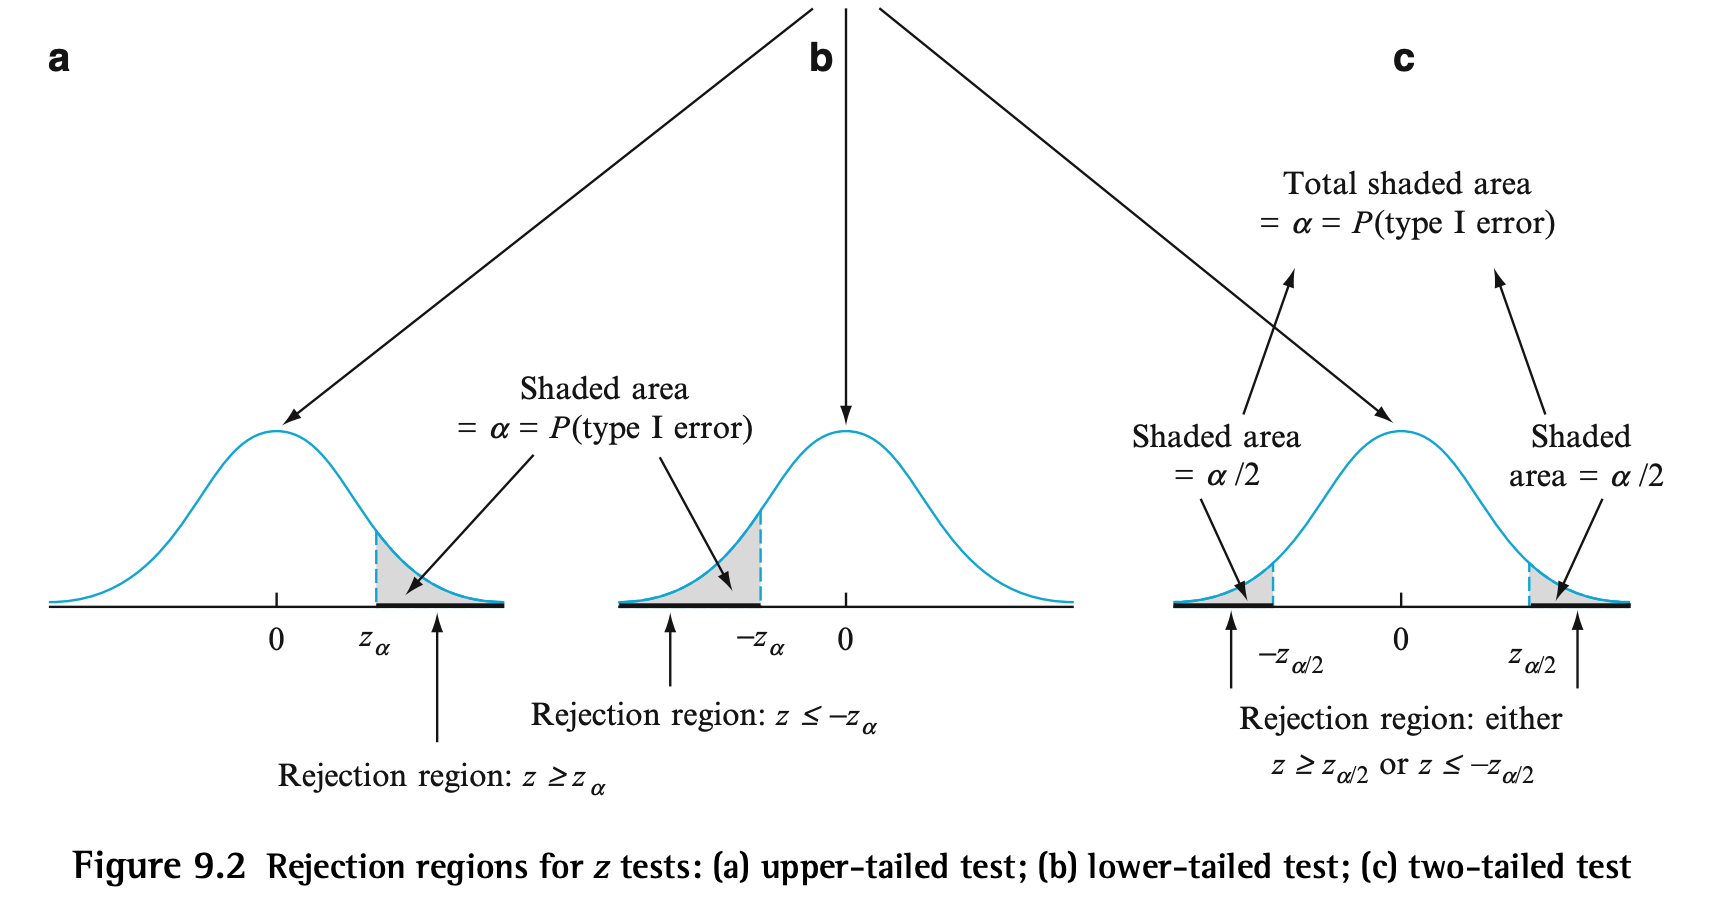
\includegraphics{images/rejectionregion.png}

}

\end{figure}
\end{frame}

\begin{frame}{Steps for Hypothesis Testing}
\protect\hypertarget{steps-for-hypothesis-testing}{}
\begin{enumerate}[<+->]
\tightlist
\item
  Identify the parameter of interest and describe it in the context of
  the problem situation.
\item
  Determine the null value and state the null hypothesis.
\item
  State the appropriate alternative hypothesis.
\item
  Give the formula for the computed value of the test statistic
  (substituting the null value and the known values of any other
  parameters, but \emph{not} those of any sample-based quantities).
\item
  State the rejection region for the selected significance level
  \(\alpha\).
\item
  Compute any necessary sample quantities, substitute into the formula
  for the test statistic value, and compute that value.
\item
  Decide whether \(H_{0}\) should be rejected and state this conclusion
  in the problem context.
\end{enumerate}
\end{frame}

\begin{frame}{Exercise 18}
\protect\hypertarget{exercise-18}{}
Reconsider the paint-drying situation of Example 9.2, in which drying
time for a test specimen is normally distributed with \(\sigma = 9\).
The hypotheses \(H_{0}: \mu = 75\) versus \(H_{a}: \mu < 75\) are to be
tested using a random sample of \(n = 25\) observations.

\begin{enumerate}[<+->]
[a.]
\tightlist
\item
  How many standard deviations (of \(\bar{X}\)) below the null value is
  \(\bar{x} = 72.3\)?
\item
  If \(\bar{x} = 72.3\), what is the conclusion using \(\alpha = 0.01\)?
\item
  What is \(\alpha\) for the test procedure that rejects \(H_{0}\) when
  \(z \leq 2.88\)?
\end{enumerate}
\end{frame}

\begin{frame}{Exercise 18 Solutions}
\protect\hypertarget{exercise-18-solutions}{}
\begin{enumerate}[<+->]
[a.]
\tightlist
\item
\end{enumerate}

\[
\begin{aligned}
z &= \frac{\bar{x} - \mu_{0}}{\sigma/\sqrt{n}} \\
&= \frac{72.3 - 75}{9/\sqrt{25}} \\
&= -1.5
\end{aligned}
\]

Therefore, \(\bar{x} = 72.3\) is 1.5 standard deviations of \(\bar{X}\)
below the null value.
\end{frame}

\begin{frame}{Exercise 18 Solutions}
\protect\hypertarget{exercise-18-solutions-1}{}
\begin{enumerate}[<+->]
[a.]
\setcounter{enumi}{1}
\tightlist
\item
\end{enumerate}

\begin{enumerate}[<+->]
\tightlist
\item
  \(\mu\) = true mean drying time for a test specimen (minutes)
\item
  \(H_{0}: \mu = 75\)
\item
  \(H_{a}: \mu < 75\)
\item
  \(z = \frac{\bar{x} - 75}{9/\sqrt{n}}\)
\item
  Using a test with significance level \(\alpha = 0.01\), \(H_{0}\) will
  be rejected if \(z \leq -z_{0.01} = -2.33\).
\item
  With \(n=25\) and \(\bar{x} = 72.3\), \(z = -1.5\) (calculated in a).
\item
  Since \(z = -1.5 \nleq -2.33\), we fail to reject \(H_{0}\) for
  \(H_{a}\). There is no statistical evidence to conclude that the true
  mean drying time for a specimen is less than 75 minutes.
\end{enumerate}
\end{frame}

\begin{frame}{Exercise 18 Solutions}
\protect\hypertarget{exercise-18-solutions-2}{}
\begin{enumerate}[<+->]
[a.]
\setcounter{enumi}{2}
\tightlist
\item
\end{enumerate}

\(\alpha\) = the area under standard normal curve below -2.88 =
\(\Phi(-2.88) = 0.0020\).
\end{frame}

\begin{frame}{\(\beta\) and Sample Size Determination}
\protect\hypertarget{beta-and-sample-size-determination}{}
The great thing about the simplicity of Case 1: There are simple
formulas for \(\beta\)!

Let's consider the upper tailed test with rejection region
\(z \geq z_{\alpha}\). This is equivalent to
\(\bar{x} \geq \mu_{0} + z_{\alpha}\sigma/\sqrt{n}\), so \(H_{0}\) will
not be rejected if \(\bar{x} < \mu_{0} + z_{\alpha}\sigma/\sqrt{n}\).

Now let \(\mu^{\prime}\) denote a particular value of \(\mu\) that
exceeds the null value \(\mu_{0}\). Then,

\[
\begin{aligned}
\beta(\mu^{\prime}) &= P(H_{0} \text{ is not rejected when } \mu = \mu^{\prime}) \\
&= P(\bar{X} < \mu_{0} + z_{\alpha}\sigma/\sqrt{n} \text{ when } \mu=\mu^{\prime}) \\
&= P\left( \frac{\bar{X} - \mu^{\prime}}{\sigma/\sqrt{n}} < z_{\alpha} + \frac{\mu_{0} - \mu^{\prime}}{\sigma/\sqrt{n}} \text{ when } \mu = \mu^{\prime}\right) \\
&= \Phi\left(z_{\alpha} + \frac{\mu_{0} - \mu^{\prime}}{\sigma/\sqrt{n}} \right)
\end{aligned}
\]
\end{frame}

\begin{frame}{\(\beta\) Determination}
\protect\hypertarget{beta-determination}{}
As \(\mu^{\prime}\) increases, \(\mu_{0} - \mu^{\prime}\) becomes more
negative, so \(\beta(\mu^{\prime})\) will be small when \(\mu^{\prime}\)
greatly exceeds \(\mu_{0}\).

We can similarly derive the formulas for lower-tailed tests and
two-tailed tests.

Try it out!
\end{frame}

\begin{frame}{Sample Size Determination}
\protect\hypertarget{sample-size-determination}{}
We found that for an upper-tailed test,

\[
\Phi\left(z_{\alpha} +  \frac{\mu_{0} - \mu^{\prime}}{\sigma/\sqrt{n}} \right) = \beta
\]

So,

\[
- z_{\beta} = z_{\alpha} +  \frac{\mu_{0} - \mu^{\prime}}{\sigma/\sqrt{n}}
\]

Where \(-z_{\beta}\) is the z critical value that captures lower tail
area \(\beta\).

This is easy to rearrange for \(n\). Try it out!
\end{frame}

\begin{frame}{\(\beta\) and Sample Size Determination}
\protect\hypertarget{beta-and-sample-size-determination-1}{}
\begin{tcolorbox}[enhanced jigsaw, left=2mm, breakable, bottomrule=.15mm, colframe=quarto-callout-important-color-frame, arc=.35mm, leftrule=.75mm, colbacktitle=quarto-callout-important-color!10!white, titlerule=0mm, opacityback=0, coltitle=black, opacitybacktitle=0.6, colback=white, toprule=.15mm, toptitle=1mm, bottomtitle=1mm, title=\textcolor{quarto-callout-important-color}{\faExclamation}\hspace{0.5em}{\(\beta\) and Sample Size}, rightrule=.15mm]

\begin{longtable}[]{@{}
  >{\raggedright\arraybackslash}p{(\columnwidth - 2\tabcolsep) * \real{0.3239}}
  >{\raggedright\arraybackslash}p{(\columnwidth - 2\tabcolsep) * \real{0.6761}}@{}}
\toprule()
\begin{minipage}[b]{\linewidth}\raggedright
\textbf{Alternative Hypothesis}
\end{minipage} & \begin{minipage}[b]{\linewidth}\raggedright
\textbf{Type II Error Probability}
\(\boldsymbol\beta(\boldsymbol\mu^{\boldsymbol\prime})\) \textbf{for a
level} \(\boldsymbol\alpha\) \textbf{test}
\end{minipage} \\
\midrule()
\endhead
\(H_{a}: \mu > \mu_{0}\) &
\(\Phi\left(z_{\alpha} + \frac{\mu_{0} - \mu^{\prime}}{\sigma/\sqrt{n}} \right)\) \\
\(H_{a}: \mu < \mu_{0}\) & 1 -
\(\Phi\left(-z_{\alpha} + \frac{\mu_{0} - \mu^{\prime}}{\sigma/\sqrt{n}} \right)\) \\
\(H_{a}: \mu \neq \mu_{0}\) &
\(\Phi\left(z_{\alpha/2} + \frac{\mu_{0} - \mu^{\prime}}{\sigma/\sqrt{n}} \right) - \Phi\left(-z_{\alpha/2} + \frac{\mu_{0} - \mu^{\prime}}{\sigma/\sqrt{n}} \right)\) \\
\bottomrule()
\end{longtable}

The sample size \(n\) for which a level \(\alpha\) test also has
\(\beta(\mu^{\prime}) = \beta\) at the alternative value
\(\mu^{\prime}\) is

\[
n = \begin{cases}
\left[\frac{\sigma(z_{\alpha} + z_{\beta})}{\mu_{0}-\mu^{\prime}}  \right]^{2} & \text{ for a one-tailed test} \\
\left[\frac{\sigma(z_{\alpha/2} + z_{\beta})}{\mu_{0}-\mu^{\prime}}  \right]^{2} & \text{ for a two-tailed test} 
\end{cases}
\]

\end{tcolorbox}
\end{frame}

\begin{frame}{Exercise 18}
\protect\hypertarget{exercise-18-1}{}
\begin{enumerate}[<+->]
[a.]
\setcounter{enumi}{3}
\tightlist
\item
  For the test procedure of part (c), what is \(\beta(70)\)?
\item
  If the test procedure of part (c) is used, what \(n\) is necessary to
  ensure that \(\beta(70) = 0.01\).
\item
  If a level 0.01 test is used with \(n=100\), what is the probability
  of a type I error when \(\mu = 76?\).
\end{enumerate}
\end{frame}

\begin{frame}{Exercise 18 Solutions}
\protect\hypertarget{exercise-18-solutions-3}{}
\begin{enumerate}[<+->]
[a.]
\setcounter{enumi}{3}
\tightlist
\item
\end{enumerate}

\[
\begin{aligned}
\beta(70) &= 1 - \Phi\left(-z_{\alpha} + \frac{\mu_{0} - \mu^{\prime}}{\sigma/\sqrt{n}}\right) \\
&= 1 - \Phi\left(-z_{0.002} + \frac{75 - 70}{9/\sqrt{25}}\right) \\
&= 1 - \Phi\left(-2.88 + \frac{75 - 70}{9/\sqrt{25}}\right)\\
&= 1 - \Phi(-0.10) \\
&= 1 - 0.4602 \\
&= 0.5398
\end{aligned}
\]
\end{frame}

\begin{frame}{Exercise 18 Solutions}
\protect\hypertarget{exercise-18-solutions-4}{}
\begin{enumerate}[<+->]
[a.]
\setcounter{enumi}{4}
\tightlist
\item
\end{enumerate}

\[
\begin{aligned}
n &= \left[\frac{\sigma(z_{\alpha} + z_{\beta})}{\mu_{0}-\mu^{\prime}}  \right]^{2} \\
&= \left[\frac{9(z_{0.0020} + z_{0.01})}{75-70}\right]^{2}\\
&= \left[\frac{9(2.88 + 2.33)}{75-70}\right]^{2} \\
&= 87.95
\end{aligned}
\]

So, \(n = 88\).
\end{frame}

\begin{frame}{Exercise 18 Solutions}
\protect\hypertarget{exercise-18-solutions-5}{}
\begin{enumerate}[<+->]
[a.]
\setcounter{enumi}{5}
\tightlist
\item
\end{enumerate}

Trick question! Type I error occurs when \(H_{0}\) is true, so if
\(\mu =76\), \(H_{0}\) is not true, so a Type I error is impossible.
Therefore the probability of making a type I error in this case is 0.
\end{frame}

\begin{frame}{Case 2: Large Sample Tests}
\protect\hypertarget{case-2-large-sample-tests}{}
We will use similar logic to large sample confidence intervals from
chapter 8. When the sample size is large, the \(z\) tests for Case 1 are
easily modified to yield valid test procedures without requiring either
a normal population distribution or known \(\sigma\).

Recall from Chapter 8, a large \(n\) implies that the sample standard
deviation \(s\) will be close to \(\sigma\) for most samples, so that
the standardized variable

\[
Z = \frac{\bar{X} - \mu}{s/\sqrt{n}}
\]

has \emph{approximately} a standard normal distribution.
\end{frame}

\begin{frame}{Large Sample Tests}
\protect\hypertarget{large-sample-tests}{}
So! We can use the same procedure for hypothesis testing as for case 1,
only substituting in \(s\) for \(\sigma\) when \(n\) is large enough.
Our rule of thumb is \(n > 40\) is large enough.

Note: Determination of \(\beta\) and the necessary sample size for these
large sample tests can be based on either specifying a plausible value
of \(\sigma\) and using the Case 1 formulas (even though \(s\) is used
in the test) or on using the methods to be introduced shortly in
connection with case 3.
\end{frame}

\begin{frame}{Exercise 20}
\protect\hypertarget{exercise-20}{}
Lightbulbs of a certain type are advertised as having an average
lifetime of 750 h. The price of these bulbs is very favorable, so a
potential customer has decided to go ahead with a purchase arrangement
unless it can be conclusively demonstrated that the true average
lifetime is smaller than what is advertised. A random sample of 50 bulbs
was~selected, the lifetime of each bulb determined. From this sample, we
found that \(\bar{x} = 738.44\) and \(s = 38.20\). Test the appropriate
hypotheses at 0.05 significance level.
\end{frame}

\begin{frame}{Case 3: A Normal Population Distribution with Unknown
\(\sigma\)}
\protect\hypertarget{case-3-a-normal-population-distribution-with-unknown-sigma}{}
When \(n\) is small, the CLT can no longer be invoked to justify the use
of a large-sample test. The same situation happened in Chapter 8 when we
were considering confidence intervals. We will take the same approach
here too.

The key result on which tests for a normal population mean are based was
used in Chapter 8 to derive the one sample t CI. If
\(X_{1}\),\ldots,\(X_{n}\) is a random sample from a normal
distribution, the standardized variable

\[
T = \frac{\bar{X} - \mu}{S/\sqrt{n}}
\]

has a \(t\) distribution with \(n-1\) degrees of freedom.
\end{frame}

\begin{frame}{Case 3}
\protect\hypertarget{case-3}{}
Consider testing \(H_{0}: \mu = \mu_{0}\) against
\(H_{a}: \mu > \mu_{0}\) by using the test statistic
\((\bar{X} - \mu_{0})/(S/\sqrt{n})\). That is, the test statistic
results from standardizing \(\bar{X}\) under the assumption that
\(H_{0}\) is true. When \(H_{0}\) is true, the test statistic has a
\(t\) distribution with \(n-1\) degrees of freedom.

Let's consider using the rejection region \(t \geq t_{\alpha,n-1}\).
This implies that

\[
\begin{aligned}
P(\text{type I error}) &= P(H_{0} \text{ is rejected when it is true}) \\
&= P(T \geq t_{\alpha,n-1} \text{ when } T \text{ has a } t \text{ distribution with } n-1 \text{ df}) \\ 
&= \alpha
\end{aligned}
\]
\end{frame}

\begin{frame}{Case 3}
\protect\hypertarget{case-3-1}{}
\begin{tcolorbox}[enhanced jigsaw, left=2mm, breakable, bottomrule=.15mm, colframe=quarto-callout-important-color-frame, arc=.35mm, leftrule=.75mm, colbacktitle=quarto-callout-important-color!10!white, titlerule=0mm, opacityback=0, coltitle=black, opacitybacktitle=0.6, colback=white, toprule=.15mm, toptitle=1mm, bottomtitle=1mm, title=\textcolor{quarto-callout-important-color}{\faExclamation}\hspace{0.5em}{The One-Sample t-Test}, rightrule=.15mm]

Null Hypothesis: \(H_{0}: \mu = \mu_{0}\) Test statistic value:
\(t = \frac{\bar{x}\ \mu_{0}}{s/\sqrt{n}}\)

\begin{longtable}[]{@{}
  >{\raggedright\arraybackslash}p{(\columnwidth - 2\tabcolsep) * \real{0.3472}}
  >{\raggedright\arraybackslash}p{(\columnwidth - 2\tabcolsep) * \real{0.6528}}@{}}
\toprule()
\begin{minipage}[b]{\linewidth}\raggedright
\textbf{Alternative Hypothesis}
\end{minipage} & \begin{minipage}[b]{\linewidth}\raggedright
\textbf{Rejection Region for Level} \(\boldsymbol\alpha\) \textbf{test}
\end{minipage} \\
\midrule()
\endhead
\(H_{a}: \mu > \mu_{0}\) & \(t > t_{\alpha,n-1}\) (upper-tailed test) \\
\(H_{a}: \mu < \mu_{0}\) & \(t < -t_{\alpha,n-1}\) (lower-tailed
test) \\
\(H_{a}: \mu \neq \mu_{0}\) & either \(t > t_{\alpha/2,n-1}\) or
\(t < -t_{\alpha/2,n-1}\) (two-tailed test) \\
\bottomrule()
\end{longtable}

\end{tcolorbox}
\end{frame}

\begin{frame}{Exercise 24}
\protect\hypertarget{exercise-24}{}
Reconsider the sample observations on stabilized viscosity of asphalt
specimens introduced in Exercise 43 in Chapter 1 (2781, 2900, 3013,
2856, and 2888). Suppose that for a particular application, it is
required that true average viscosity be 3000. Does this requirement
appear to have been satisfied? State and test the appropriate
hypotheses.

\(\bar{x} = 2887.6\) \(s = 84.0256\) \(n = 5\)
\end{frame}

\begin{frame}{Exercise 24 Solutions}
\protect\hypertarget{exercise-24-solutions}{}
\begin{enumerate}[<+->]
\tightlist
\item
  \(\mu\) = the true average viscosity of asphalt
\item
  \(H_{0}: \mu = 3000\)
\item
  \(H_{a}: \mu \neq 3000\)
\item
  \(t = \frac{\bar{x} - 3000}{s/\sqrt{n}}\)
\item
  Using a test with significance level \(0.05\), \(H_{0}\) will be
  rejected if \(t \geq t_{0.025, 4} = 2.776\) or \(t \leq - 2.776\)
\item
  \(t = \frac{\bar{x} - 3000}{s/\sqrt{n}} = \frac{2887.6 - 3000}{84.0256/\sqrt{5}} = -2.991\)
\item
  Reject \(H_{0}\) since \(t = -2.991 \leq -2.776\). Therefore, at 5\%
  significance, we have enough statistical evidence to conclude that the
  true average viscosity of the asphalt is not 3000. The requirement is
  not met.
\end{enumerate}
\end{frame}

\begin{frame}{\(\beta\) and Sample Size Determination}
\protect\hypertarget{beta-and-sample-size-determination-2}{}
The calculation of \(\beta(\mu^{\prime})\) is much less straightforward
for the \(t\) test than it was for Case 1. This is because the
distribution of the test statistic is quite complicated when \(H_{0}\)
is false and \(H_{a}\) is true.

So, for an upper tailed test for example, determining

\[ 
\beta(\mu^{\prime}) = P(T < t_{\alpha,n-1} \text{ when } \mu = \mu^{\prime} \text{ rather than }\mu_{0})
\]

involves integrating a very unpleasant density function. This must be
done numerically (with computer software!) or by looking at the graphs
in Appendix Table A.16. There are four graphs corresponding to
one-tailed tests at level 0.05 and 0.01, and two-tailed tests at the
same levels.
\end{frame}

\begin{frame}{\(\beta\) and Sample Size Determination}
\protect\hypertarget{beta-and-sample-size-determination-3}{}
The graphs are in terms of \(\beta\) on the vertical axis and \(d\) on
the horizontal axis, where \(d = |\mu_{0} - \mu^{\prime}|/\sigma\).

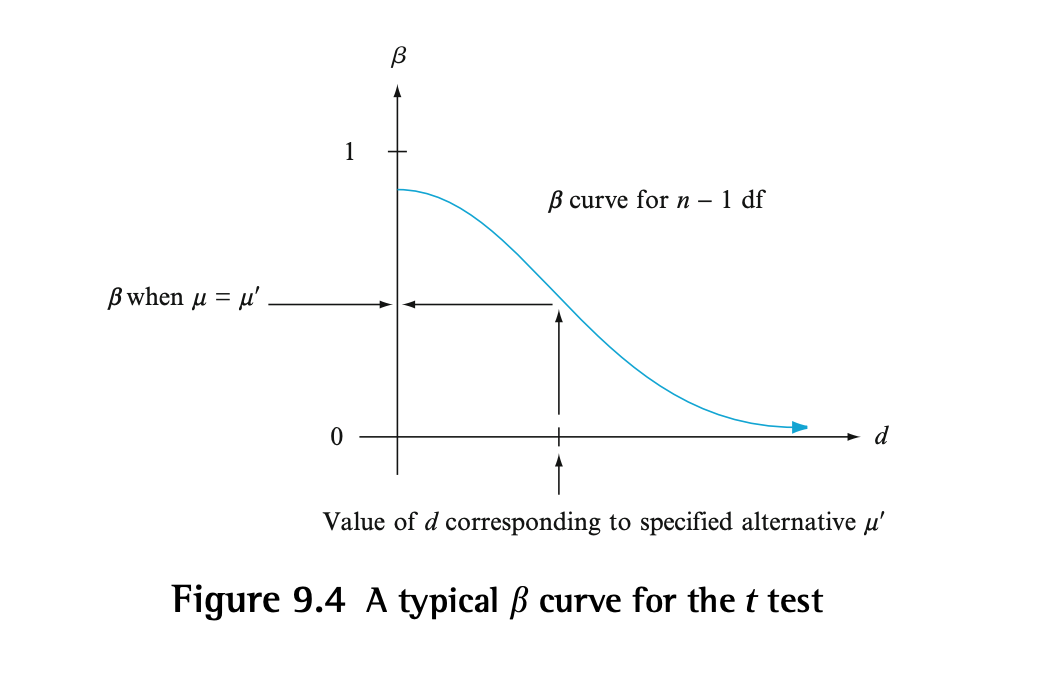
\includegraphics{images/betacurve.png}

Similarly, we can use the table to help us determine sample size. Let's
see it in an example.
\end{frame}

\begin{frame}{Exercise 32}
\protect\hypertarget{exercise-32}{}
A sample of 12 radon detectors of a certain type was selected and each
was exposed to 100 pCi/L of radon. The resulting readings were as
follows:

\begin{longtable}[]{@{}llllll@{}}
\toprule()
\endhead
105.6 & 90.9 & 91.2 & 96.9 & 96.5 & 91.3 \\
100.1 & 105.0 & 99.6 & 107.7 & 103.3 & 92.4 \\
\bottomrule()
\end{longtable}

\begin{enumerate}[<+->]
[a.]
\tightlist
\item
  Does this data suggest that the population mean reading under these
  conditions differs from 100? State and test the appropriate hypotheses
  using \(\alpha = 0.05\).
\item
  Suppose that prior to the experiment, a value of \(\sigma = 7.5\) had
  been assumed. How many determinations would then have been appropriate
  to obtain \(\beta = 0.10\) for the alternative \(\mu = 95\)?
\end{enumerate}
\end{frame}

\begin{frame}{Summary}
\protect\hypertarget{summary-2}{}
\begin{itemize}[<+->]
\tightlist
\item
  Case 1:
\end{itemize}

Null Hypothesis: \(H_{0}: \mu = \mu_{0}\)\\
Test Statistic value: \(z = \frac{\bar{x} - \mu_{0}}{\sigma/\sqrt{n}}\)

\begin{longtable}[]{@{}
  >{\raggedright\arraybackslash}p{(\columnwidth - 2\tabcolsep) * \real{0.3611}}
  >{\raggedright\arraybackslash}p{(\columnwidth - 2\tabcolsep) * \real{0.6389}}@{}}
\toprule()
\begin{minipage}[b]{\linewidth}\raggedright
\textbf{Alternative Hypothesis}
\end{minipage} & \begin{minipage}[b]{\linewidth}\raggedright
\textbf{Rejection Region for Level} \(\boldsymbol\alpha\) \textbf{test}
\end{minipage} \\
\midrule()
\endhead
\(H_{a}: \mu > \mu_{0}\) & \(z > z_{\alpha}\) (upper-tailed test) \\
\(H_{a}: \mu < \mu_{0}\) & \(z < -z_{\alpha}\) (lower-tailed test) \\
\(H_{a}: \mu \neq \mu_{0}\) & either \(z > z_{\alpha/2}\) or
\(z < -z_{\alpha/2}\) (two-tailed test) \\
\bottomrule()
\end{longtable}

\begin{itemize}[<+->]
\tightlist
\item
  Case 2: We can use all the same procedures and formulas for case 1,
  only substituting in \(s\) for \(\sigma\) when \(n\) is large enough.
  Our rule of thumb is \(n > 40\) is large enough.
\end{itemize}
\end{frame}

\begin{frame}{Summary}
\protect\hypertarget{summary-3}{}
\begin{itemize}[<+->]
\tightlist
\item
  Case 3:
\end{itemize}

Null Hypothesis: \(H_{0}: \mu = \mu_{0}\)\\
Test statistic value: \(t = \frac{\bar{x}\ \mu_{0}}{s/\sqrt{n}}\)

\begin{longtable}[]{@{}
  >{\raggedright\arraybackslash}p{(\columnwidth - 2\tabcolsep) * \real{0.3611}}
  >{\raggedright\arraybackslash}p{(\columnwidth - 2\tabcolsep) * \real{0.6389}}@{}}
\toprule()
\begin{minipage}[b]{\linewidth}\raggedright
\textbf{Alternative Hypothesis}
\end{minipage} & \begin{minipage}[b]{\linewidth}\raggedright
\textbf{Rejection Region for Level} \(\boldsymbol\alpha\) \textbf{test}
\end{minipage} \\
\midrule()
\endhead
\(H_{a}: \mu > \mu_{0}\) & \(t > t_{\alpha,n-1}\) (upper-tailed test) \\
\(H_{a}: \mu < \mu_{0}\) & \(t < -t_{\alpha,n-1}\) (lower-tailed
test) \\
\(H_{a}: \mu \neq \mu_{0}\) & either \(t > t_{\alpha/2,n-1}\) or
\(t < -t_{\alpha/2,n-1}\) (two-tailed test) \\
\bottomrule()
\end{longtable}
\end{frame}

\begin{frame}{Practice Problems}
\protect\hypertarget{practice-problems-1}{}
\begin{itemize}[<+->]
\tightlist
\item
  Odd problems 15 - 31
\item
  35
\end{itemize}
\end{frame}

\hypertarget{tests-concerning-a-population-proportion}{%
\section{9.3 Tests Concerning a Population
Proportion}\label{tests-concerning-a-population-proportion}}

\begin{frame}{Outcomes}
\protect\hypertarget{outcomes-2}{}
By the end of this section, you will be able to:

\begin{itemize}[<+->]
\tightlist
\item
  Use general large sample tests for parameter \(\theta\) following
  certain conditions.
\item
  Perform all steps of a large sample z test for \(p\).
\item
  Calculate \(\beta\) and \(n\) from a large sample \(z\) test for
  \(p\).
\item
  Perform all steps of a small sample test for \(p\).
\end{itemize}
\end{frame}

\begin{frame}{Large Sample Tests}
\protect\hypertarget{large-sample-tests-1}{}
\begin{itemize}[<+->]
\tightlist
\item
  Large-sample tests concerning \(p\) are a special case of the more
  general large-sample procedures for a parameter \(\theta\).
\item
  Let \(\hat{\theta}\) be an estimator of \(\theta\) that is
  approximately unbiased and has approximately a normal distribution.
\item
  The null hypothesis has the form \(H_{0}: \theta = \theta_{0}\) where
  \(\theta_{0}\) denotes a number (the null value) appropriate to the
  problem context.
\item
  Suppose that when \(H_{0}\) is true, the standard deviation of
  \(\hat{\theta}\), \(\sigma_{\hat{\theta}}\) involves no unknown
  parameters.
\item
  A large-sample test statistic results from standardizing
  \(\hat{\theta}\) under the assumption that \(H_{0}\) is true:
\end{itemize}

\[
\text{Test Statistic} = \frac{\hat{\theta} - \theta_{0}}{\sigma_{\hat{\theta}}} 
\]
\end{frame}

\begin{frame}{Large Sample Tests}
\protect\hypertarget{large-sample-tests-2}{}
\begin{itemize}[<+->]
\tightlist
\item
  If the alternative hypothesis is \(H_{a}: \theta > \theta_{0}\), an
  upper-tailed test whose significance level is approximately \(\alpha\)
  is specified by the rejection region \(z \geq z_{\alpha}\).
\item
  Similarly, we can work out the rejection regions for the other two
  alternatives.
\end{itemize}
\end{frame}

\begin{frame}{Case of \(\theta = p\)}
\protect\hypertarget{case-of-theta-p}{}
\begin{itemize}[<+->]
\tightlist
\item
  In the case of \(\theta = p\), \(\sigma_{\hat{\theta}}\) will not
  involve any unknown parameters when \(H_{0}\) is true, but this is
  atypical.
\item
  When \(\sigma_{\hat{\theta}}\) does involve unknown parameters, it is
  often possible to use an estimated standard deviation
  \(S_{\hat{\theta}}\) in place of \(\sigma_{\hat{\theta}}\) and still
  have \(Z\) approximately normally distributed when \(H_{0}\) is true
  (because when \(n\) is large,
  \(s_{\hat{\theta}} \approx \sigma_{\hat{\theta}}\) for most samples).
\item
  The large-sample test of the previous section furnishes an example of
  this: Because \(\sigma\) is usually unknown, we use
  \(s_{\hat{\theta}} = s_{\bar{x}} = s/\sqrt{n}\) in place of
  \(\sigma/\sqrt{n}\) in the denominator of \(z\).
\end{itemize}
\end{frame}

\begin{frame}{Case of \(\theta = p\)}
\protect\hypertarget{case-of-theta-p-1}{}
\begin{itemize}[<+->]
\tightlist
\item
  The estimator \(\hat{p} = X/n\) is unbiased, has approximately a
  normal distribution, and it's standard deviation is
  \(\sigma_{\hat{p}} = \sqrt{p(1-p)/n}\).
\item
  When \(H_{0}\) is true, \(E(\hat{p}) = p_{0}\) and
  \(\sigma_{\hat{p}} = \sqrt{p_{0}(1-p_{0})/n}\), so
  \(\sigma_{\hat{p}}\) does not involve any unknown parameters.
\item
  It then follows that when \(n\) is large and \(H_{0}\) is true, the
  test statistic
\end{itemize}

\[
Z = \frac{\hat{p} - p_{0}}{\sqrt{p_{0}(1-p_{0})/n}}
\]

has approximately a standard normal distribution.
\end{frame}

\begin{frame}{Case of \(\theta = p\)}
\protect\hypertarget{case-of-theta-p-2}{}
\begin{itemize}[<+->]
\tightlist
\item
  If the alternative hypothesis is \(H_{a}: p > p_{0}\) and the upper
  tailed rejection region \(z \geq z_{\alpha}\) is used, then
\end{itemize}

\[
\begin{aligned}
P(\text{type I error}) &= P(H_{0} \text{ is rejected when it is true}) \\
&= P(Z \geq z_{\alpha} \text{ when Z has approximately a standard} \\
&\text{normal distribution}) \\
&\approx \alpha
\end{aligned}
\]

\begin{itemize}[<+->]
\tightlist
\item
  Thus the desired level of significance \(\alpha\) is attained by using
  the critical value that captures area \(\alpha\) in the upper tail of
  the \(z\) curve.
\item
  Rejection regions for the other two alternative hypotheses are
  justified in an analogous manner.
\end{itemize}
\end{frame}

\begin{frame}{Large sample test for p}
\protect\hypertarget{large-sample-test-for-p}{}
\begin{tcolorbox}[enhanced jigsaw, left=2mm, breakable, bottomrule=.15mm, colframe=quarto-callout-important-color-frame, arc=.35mm, leftrule=.75mm, colbacktitle=quarto-callout-important-color!10!white, titlerule=0mm, opacityback=0, coltitle=black, opacitybacktitle=0.6, colback=white, toprule=.15mm, toptitle=1mm, bottomtitle=1mm, title=\textcolor{quarto-callout-important-color}{\faExclamation}\hspace{0.5em}{Important}, rightrule=.15mm]

Null hypothesis: \(H_{0}: p = p_{0}\)\\
Test statistic value:
\(z = \frac{\hat{p} - p_{0}}{\sqrt{p_{0}(1-p_{0})/n}}\)

\begin{longtable}[]{@{}
  >{\raggedright\arraybackslash}p{(\columnwidth - 2\tabcolsep) * \real{0.3472}}
  >{\raggedright\arraybackslash}p{(\columnwidth - 2\tabcolsep) * \real{0.6528}}@{}}
\toprule()
\begin{minipage}[b]{\linewidth}\raggedright
\textbf{Alternative Hypothesis}
\end{minipage} & \begin{minipage}[b]{\linewidth}\raggedright
\textbf{Rejection Region}
\end{minipage} \\
\midrule()
\endhead
\(H_{a}: p > p_{0}\) & \(z \geq z_{\alpha}\) (upper-tailed) \\
\(H_{a}: p < p_{0}\) & \(z \leq z_{\alpha}\) (lower-tailed) \\
\(H_{a}: p \neq p_{0}\) & either \(z \geq z_{\alpha/2}\) or
\(z \leq -z_{\alpha/2}\) (two-tailed) \\
\bottomrule()
\end{longtable}

\end{tcolorbox}
\end{frame}

\begin{frame}{Exercise 36}
\protect\hypertarget{exercise-36}{}
State DMV records indicate that of all vehicles undergoing emissions
testing during the previous year, 70\% passed on the first try. A random
sample of 200 cars tested in a particular county during the current year
yields 124 that passed on the initial test. Does this suggest that the
true proportion for this county during the current year differs from the
previous statewide proportion? Test the relevant hypotheses using
\(\alpha = 0.05\).
\end{frame}

\begin{frame}{Exercise 36 Solutions}
\protect\hypertarget{exercise-36-solutions}{}
\begin{enumerate}[<+->]
\tightlist
\item
  \(p\) = true proportion of vehicles in a particular county during the
  current year that passed emissions test on the first try.
\item
  \(H_{0}: p = 0.70\)
\item
  \(H_{a}: p \neq 0.70\)
\item
  \(Z = \frac{\hat{p} - 0.70}{\sqrt{0.7(0.3)/n}}\)
\item
  Reject \(H_{0}\) if \(z \geq z_{0.05/2} = 1.96\) or \(z \leq - 1.96\).
\item
  \(z = \frac{(124/200) - 0.70}{\sqrt{0.7(0.3)/200}} = -2.47\)
\item
  Reject \(H_{0}\) for \(H_{a}\) since \(z = -2.47 \geq -1.96\).
  Therefore, at 5\% significance, we have enough evidence to conclude
  that the true proportion of vehicles in a particular county during the
  current year that passe emissions test on the first try differs from
  that of the previous statewide proportion of 0.70.
\end{enumerate}
\end{frame}

\begin{frame}{\(\beta\) and Sample Size Determination}
\protect\hypertarget{beta-and-sample-size-determination-4}{}
\begin{itemize}[<+->]
\tightlist
\item
  When \(H_{0}\) is true, the test statistic \(Z\) has approximately a
  standard normal distribution.
\item
  Now suppose that \(H_{0}\) is not true, and that \(p = p^{\prime}\).
\item
  Then \(Z\) still has approximately a normal distribution (because it
  is a linear function of \(\hat{p}\)) but its mean value and variance
  are no loner 0 and 1 respectively.
\item
  Instead,
\end{itemize}

\[
E(Z) = \frac{p^{\prime} - p_{0}}{\sqrt{p_{0}(1-p_{0})/n}} \hspace{2cm} V(Z) = \frac{p^{\prime}(1-p^{\prime})/n}{p_{0}(1-p_{0})/n}
\]
\end{frame}

\begin{frame}{\(\beta\) and Sample Size Determination}
\protect\hypertarget{beta-and-sample-size-determination-5}{}
\begin{itemize}[<+->]
\tightlist
\item
  The probability of a type II error for an upper-tailed test is
  \(\beta(p^{\prime}) = P(Z < z_{\alpha} \text{ when } p = p^{\prime})\).
\item
  This can be computed by using the given mean and variance to
  standardize and then referring to the standard normal cdf.
\item
  In addition, if it is desired that the level \(\alpha\) test also have
  \(\beta(p^{\prime}) = \beta\) for a specified value of \(\beta\), this
  equation can be solved for the necessary \(n\).
\end{itemize}
\end{frame}

\begin{frame}{\(\beta\) and Sample Size Determination}
\protect\hypertarget{beta-and-sample-size-determination-6}{}
\begin{tcolorbox}[enhanced jigsaw, left=2mm, breakable, bottomrule=.15mm, colframe=quarto-callout-important-color-frame, arc=.35mm, leftrule=.75mm, colbacktitle=quarto-callout-important-color!10!white, titlerule=0mm, opacityback=0, coltitle=black, opacitybacktitle=0.6, colback=white, toprule=.15mm, toptitle=1mm, bottomtitle=1mm, title=\textcolor{quarto-callout-important-color}{\faExclamation}\hspace{0.5em}{\(\beta\) and \(n\)}, rightrule=.15mm]

\begin{longtable}[]{@{}
  >{\raggedright\arraybackslash}p{(\columnwidth - 2\tabcolsep) * \real{0.3239}}
  >{\raggedright\arraybackslash}p{(\columnwidth - 2\tabcolsep) * \real{0.6761}}@{}}
\toprule()
\begin{minipage}[b]{\linewidth}\raggedright
\textbf{Alternative Hypothesis}
\end{minipage} & \begin{minipage}[b]{\linewidth}\raggedright
\(\boldsymbol\beta(p^{\prime})\)
\end{minipage} \\
\midrule()
\endhead
\(H_{a}: p > p_{0}\) &
\(\Phi\left[\frac{p_{0} - p^{\prime}+z_{\alpha}\sqrt{p_{0}(1-p_{0})/n}}{\sqrt{p^{\prime}(1-p^{\prime})/n}} \right]\) \\
\(H_{a}: p < p_{0}\) &
\(1 - \Phi\left[\frac{p_{0} - p^{\prime}-z_{\alpha}\sqrt{p_{0}(1-p_{0})/n}}{\sqrt{p^{\prime}(1-p^{\prime})/n}} \right]\) \\
\(H_{a}: p \neq p_{0}\) &
\(\Phi\left[\frac{p_{0} - p^{\prime}+z_{\alpha/2}\sqrt{p_{0}(1-p_{0})/n}}{\sqrt{p^{\prime}(1-p^{\prime})/n}} \right] -\Phi\left[\frac{p_{0} - p^{\prime}-z_{\alpha/2}\sqrt{p_{0}(1-p_{0})/n}}{\sqrt{p^{\prime}(1-p^{\prime})/n}} \right]\) \\
\bottomrule()
\end{longtable}

The sample size \(n\) for which the level \(\alpha\) test also satisfies
\(\beta(p^{\prime}) = \beta\) is

\[
n = \begin{cases}
\left[\frac{z_{\alpha}\sqrt{p_{0}(1-p_{0})} + z_{\beta}\sqrt{p^{\prime}(1-p^{\prime})}}{p^{\prime} - p_{0}} \right]^{2} & \text{one-tailed test} \\
\left[\frac{z_{\alpha/2}\sqrt{p_{0}(1-p_{0})} + z_{\beta}\sqrt{p^{\prime}(1-p^{\prime})}}{p^{\prime} - p_{0}} \right]^{2} & \text{two-tailed test approximately} 
\end{cases}
\]

\end{tcolorbox}
\end{frame}

\begin{frame}{Exercise 44}
\protect\hypertarget{exercise-44}{}
Scientists have recently become concerned about the safety of Teflon
cookware and various food containers because perfluorooctanoic acid
(PFOA) is used in the manufacturing process. An article reported in the
\emph{New York Times} reported that of 600 children tested, 96\% had
PFOA in their blood. According to the FDA, 90\% of all Americans have
PFOA in their blood.

\begin{enumerate}[<+->]
[a.]
\tightlist
\item
  Does the data on PFOA incidence among children suggest that the
  percentage of all children who have PFOA in their blood exceeds the
  FDA percentage for all Americans. Carry out an appropriate hypothesis
  test at 1\% significance.
\item
  If 95\% of all children have PFOA in their blood, how likely is it
  that the null hypothesis tested in (a) will be rejected when a
  significance level of 0.01 is employed?
\item
  Referring back to (b), what sample size would be necessary for the
  relevant probability to be 0.10?
\end{enumerate}
\end{frame}

\begin{frame}{Small-Sample Tests}
\protect\hypertarget{small-sample-tests}{}
\begin{itemize}[<+->]
\tightlist
\item
  Test procedures when the sample size \(n\) is small are based directly
  on the binomial distribution rather than the normal approximation.
\item
  Consider the alternative hypothesis \(H_{a}: p < p_{0}\) and again let
  \(X\) be the number of successes in the sample.
\item
  Then \(X\) is the test statistic, and the upper-tailed rejection
  region has the form \(x \geq c\).
\item
  When \(H_{0}\) is true, \(X\) has a binomial distribution with
  parameters \(n\) and \(p_{0}\), so
\end{itemize}

\[
\begin{aligned}
P(\text{type I error}) &= P(H_{0} \text{ is rejected when it is true}) \\
&= P(X \geq c \text{ when } X \sim Bin(n,p_{0})) \\
&= 1 - P(X \leq c - 1 \text{ when } X \sim Bin(n,p_{0})) \\
&= 1 - B(c-1;n,p_{0})
\end{aligned}
\]
\end{frame}

\begin{frame}{Small-Sample Tests}
\protect\hypertarget{small-sample-tests-1}{}
\begin{itemize}[<+->]
\tightlist
\item
  As the critical value \(c\) decreases, more \(x\) values are included
  in the rejection region and \(P(\text{type I error})\) increases.
\item
  Because \(X\) has a discrete probability distribution, it is usually
  not possible to find a value of \(c\) for which
  \(P(\text{type I error})\) is exactly the desired significance level
  \(\alpha\).
\item
  Instead, the largest rejection region of the form \{c, c+1, \ldots,
  n\} satisfying \(1 - B(c-1;n,p_{0}) \leq \alpha\) is used.
\end{itemize}
\end{frame}

\begin{frame}{Small-Sample Tests}
\protect\hypertarget{small-sample-tests-2}{}
\begin{itemize}[<+->]
\tightlist
\item
  Let \(p^{\prime}\) denote the alternative value of \(p\)
  (\(p^{\prime} > p_{0}\)).
\item
  When \(p = p^{\prime}\), \(X \sim Bin(n,p^{\prime})\), so
\end{itemize}

\[
\begin{aligned}
\beta(p^{\prime}) &= P(\text{ type II error when } p = p^{\prime}) \\
&= P(X < c \text{ when } X\sim B(n,p^{\prime})) \\
&= B(c-1;n,p^{\prime})
\end{aligned}
\]

\begin{itemize}[<+->]
\tightlist
\item
  Similarly, we can construct test procedures for the other two
  alternatives.
\end{itemize}
\end{frame}

\begin{frame}{Exercise 42}
\protect\hypertarget{exercise-42}{}
Each of a group of 20 intermediate tennis players is given two rackets,
one having nylon strings and the other synthetic gut strings. After
several weeks of playing with the two rackets, each player will be asked
to state a preference for one of the two types of strings. Let \(p\)
denote the proportion of all such players who would prefer gut to nylon,
and let \(X\) be the number of players in the sample who prefer gut.
Because gut strings are more expensive, consider the null hypothesis
that at most 50\% of all such players prefer gut. We simplify this to
\(H_{0}: p = 0.5\), planning to reject \(H_{0}\) only if sample evidence
strongly favours gut strings.
\end{frame}

\begin{frame}{Exercise 42}
\protect\hypertarget{exercise-42-1}{}
\begin{enumerate}[<+->]
[a.]
\tightlist
\item
  Which of the rejection regions \{15, 16, 17, 18, 19, 20 \}, \{0, 1, 2,
  3, 4, 5\}, or \{0, 1, 2, 3, 17, 18, 19, 20 \} is most appropriate and
  why are the other two nor appropriate?
\item
  What is the probability of a type I error for the chosen region of
  part (a)? Does the region specify a level 0.05 test? Is it the best
  level 0.05 test?
\item
  If 60\% of all enthusiasts prefer gut, calculate the probability of a
  type II error using the appropriate region from part (a). Repeat if
  80\% of all enthusiasts prefer gut.
\item
  If 13 out of the 20 players prefer gut, should \(H_{0}\) be rejected
  using a significance level of 0.10?
\end{enumerate}
\end{frame}

\begin{frame}{Summary}
\protect\hypertarget{summary-4}{}
\begin{itemize}[<+->]
\tightlist
\item
  A general large sample test for parameter \(\theta\) when
  \(\hat{\theta}\) is approximately unbiased and has approximately a
  normal distribution and \(\sigma_{\hat{\theta}}\) involves no unknown
  parameters, then the test statistic
  \(Z = \frac{\hat{\theta} - \theta_{0}}{\sigma_{\hat{\theta}}}\) can be
  used.
\item
  A large sample test for \(p\) is performed as follows:\\
  Null hypothesis: \(H_{0}: p = p_{0}\)\\
  Test statistic value:
  \(z = \frac{\hat{p} - p_{0}}{\sqrt{p_{0}(1-p_{0})/n}}\)
\end{itemize}

\begin{longtable}[]{@{}
  >{\raggedright\arraybackslash}p{(\columnwidth - 2\tabcolsep) * \real{0.3611}}
  >{\raggedright\arraybackslash}p{(\columnwidth - 2\tabcolsep) * \real{0.6389}}@{}}
\toprule()
\begin{minipage}[b]{\linewidth}\raggedright
\textbf{Alternative Hypothesis}
\end{minipage} & \begin{minipage}[b]{\linewidth}\raggedright
\textbf{Rejection Region}
\end{minipage} \\
\midrule()
\endhead
\(H_{a}: p > p_{0}\) & \(z \geq z_{\alpha}\) (upper-tailed) \\
\(H_{a}: p < p_{0}\) & \(z \leq z_{\alpha}\) (lower-tailed) \\
\(H_{a}: p \neq p_{0}\) & either \(z \geq z_{\alpha/2}\) or
\(z \leq -z_{\alpha/2}\) (two-tailed) \\
\bottomrule()
\end{longtable}
\end{frame}

\begin{frame}{Summary}
\protect\hypertarget{summary-5}{}
\begin{itemize}[<+->]
\tightlist
\item
  \(\beta\) and \(n\) can be calculated from the following for a large
  sample \(z\) test for \(p\).
\end{itemize}

\begin{longtable}[]{@{}
  >{\raggedright\arraybackslash}p{(\columnwidth - 2\tabcolsep) * \real{0.3333}}
  >{\raggedright\arraybackslash}p{(\columnwidth - 2\tabcolsep) * \real{0.6667}}@{}}
\toprule()
\begin{minipage}[b]{\linewidth}\raggedright
\textbf{Alternative Hypothesis}
\end{minipage} & \begin{minipage}[b]{\linewidth}\raggedright
\(\boldsymbol\beta(p^{\prime})\)
\end{minipage} \\
\midrule()
\endhead
\(H_{a}: p > p_{0}\) &
\(\Phi\left[\frac{p_{0} - p^{\prime}+z_{\alpha}\sqrt{p_{0}(1-p_{0})/n}}{\sqrt{p^{\prime}(1-p^{\prime})/n}} \right]\) \\
\(H_{a}: p < p_{0}\) &
\(1 - \Phi\left[\frac{p_{0} - p^{\prime}-z_{\alpha}\sqrt{p_{0}(1-p_{0})/n}}{\sqrt{p^{\prime}(1-p^{\prime})/n}} \right]\) \\
\(H_{a}: p \neq p_{0}\) &
\(\Phi\left[\frac{p_{0} - p^{\prime}+z_{\alpha/2}\sqrt{p_{0}(1-p_{0})/n}}{\sqrt{p^{\prime}(1-p^{\prime})/n}} \right] -\Phi\left[\frac{p_{0} - p^{\prime}-z_{\alpha/2}\sqrt{p_{0}(1-p_{0})/n}}{\sqrt{p^{\prime}(1-p^{\prime})/n}} \right]\) \\
\bottomrule()
\end{longtable}

\begin{itemize}[<+->]
\tightlist
\item
  A small sample test for \(p\) relies on the binomial distribution
  instead of the normal approximation.
\end{itemize}
\end{frame}

\begin{frame}{Practice Problems}
\protect\hypertarget{practice-problems-2}{}
\begin{itemize}[<+->]
\tightlist
\item
  Odd problems 37 - 41
\end{itemize}
\end{frame}

\hypertarget{p-values}{%
\section{9.4 P-values}\label{p-values}}

\begin{frame}{Outcomes}
\protect\hypertarget{outcomes-3}{}
By the end of this section, you will be able to:

\begin{itemize}[<+->]
\tightlist
\item
  Define and interpret the p-value.
\item
  Calculate the p-value for all of the tests we have learned so far.
\item
  Use the p-value to perform a hypothesis test for all the tests we have
  seen so far.
\end{itemize}
\end{frame}

\begin{frame}{P-value}
\protect\hypertarget{p-value}{}
\begin{itemize}[<+->]
\tightlist
\item
  Using the rejection region method to test hypotheses entails first
  selecting a significance level \(\alpha\).
\item
  Then after computing the test statistic, the null hypothesis \(H_{0}\)
  is rejected if the value falls in the rejection region and is
  otherwise not rejected.
\item
  We now consider another way or reaching a conclusion in a hypothesis
  testing analysis.
\item
  This alternative approach is based on calculation of a certain
  probability called a \emph{p-value}.
\item
  One advantage is that the p-value provides an intuitive measure of the
  strength of evidence in the data against \(H_{0}\).
\end{itemize}
\end{frame}

\begin{frame}{P-value}
\protect\hypertarget{p-value-1}{}
\begin{tcolorbox}[enhanced jigsaw, left=2mm, breakable, bottomrule=.15mm, colframe=quarto-callout-important-color-frame, arc=.35mm, leftrule=.75mm, colbacktitle=quarto-callout-important-color!10!white, titlerule=0mm, opacityback=0, coltitle=black, opacitybacktitle=0.6, colback=white, toprule=.15mm, toptitle=1mm, bottomtitle=1mm, title=\textcolor{quarto-callout-important-color}{\faExclamation}\hspace{0.5em}{Definition}, rightrule=.15mm]

The \textbf{p-value} is the probability, calculated assuming that the
null hypothesis is true, of obtaining a value of the test statistic at
least as contradictory to \(H_{0}\) as the value calculated from the
available sample.

\end{tcolorbox}

Key points:

\begin{itemize}[<+->]
\tightlist
\item
  The p-value is a probability.
\item
  This probability is calculated assuming that the null hypothesis is
  true.
\item
  To determine the p-value, we must first decide which values of the
  test statistic are at least as contradictory to \(H_{0}\) as the value
  obtained from our sample.
\end{itemize}
\end{frame}

\begin{frame}{Exercise 48}
\protect\hypertarget{exercise-48}{}
Newly purchased tires of a certain type are supposed to be filled to a
pressure of 30 lb/in\(^{2}\). Let \(\mu\) denote the true average
pressure. Find the p-value associated with each given \(z\) statistic
value for testing \(H_{0}: mu = 30\) versus \(H_{a}: \mu \neq 30\).

\begin{enumerate}[<+->]
[a.]
\tightlist
\item
  2.10
\end{enumerate}

Okay, so we need to think about what is at least as contradictory to
\(H_{a}\) as our observed test statistic. If our sample observation
obtained exactly 30, \(z\) would be zero. So we need to be
\textbf{further away} from 0, in either direction (since we have a
two-tailed hypothesis).

Therefore,

\[
\begin{aligned}
p-value &= P(Z \geq 2.10 \text{ or } Z \leq -2.10 \text{ given } H_{0} \text{ is true}) \\
&= P(Z \geq 2.10) + P(Z \leq -2.10) \\
&= 0.0179 + 0.0179 \\
&= 0.0358
\end{aligned}
\]

Therefore, 3.58\% of all possible test statistic values are more
contradictory to \(H_{0}\) as we obtained. Thus, the sample appears to
be relatively contradictory to the null hypothesis.
\end{frame}

\begin{frame}{P-value Decisions}
\protect\hypertarget{p-value-decisions}{}
\begin{itemize}[<+->]
\tightlist
\item
  The smaller the p-value, the more evidence there is in the sample data
  against the null hypothesis and for the alternative hypothesis.
\end{itemize}

\begin{tcolorbox}[enhanced jigsaw, left=2mm, breakable, bottomrule=.15mm, colframe=quarto-callout-important-color-frame, arc=.35mm, leftrule=.75mm, colbacktitle=quarto-callout-important-color!10!white, titlerule=0mm, opacityback=0, coltitle=black, opacitybacktitle=0.6, colback=white, toprule=.15mm, toptitle=1mm, bottomtitle=1mm, title=\textcolor{quarto-callout-important-color}{\faExclamation}\hspace{0.5em}{Decision Rule based on the p-value}, rightrule=.15mm]

Select a significance level \(\alpha\) (as before, the desired type I
error probability). Then reject \(H_{0}\) if p-value \(\leq \alpha\); do
not reject \(H_{0}\) if p-value \(> \alpha\).

\end{tcolorbox}
\end{frame}

\begin{frame}{P-value Versus Rejection Region}
\protect\hypertarget{p-value-versus-rejection-region}{}
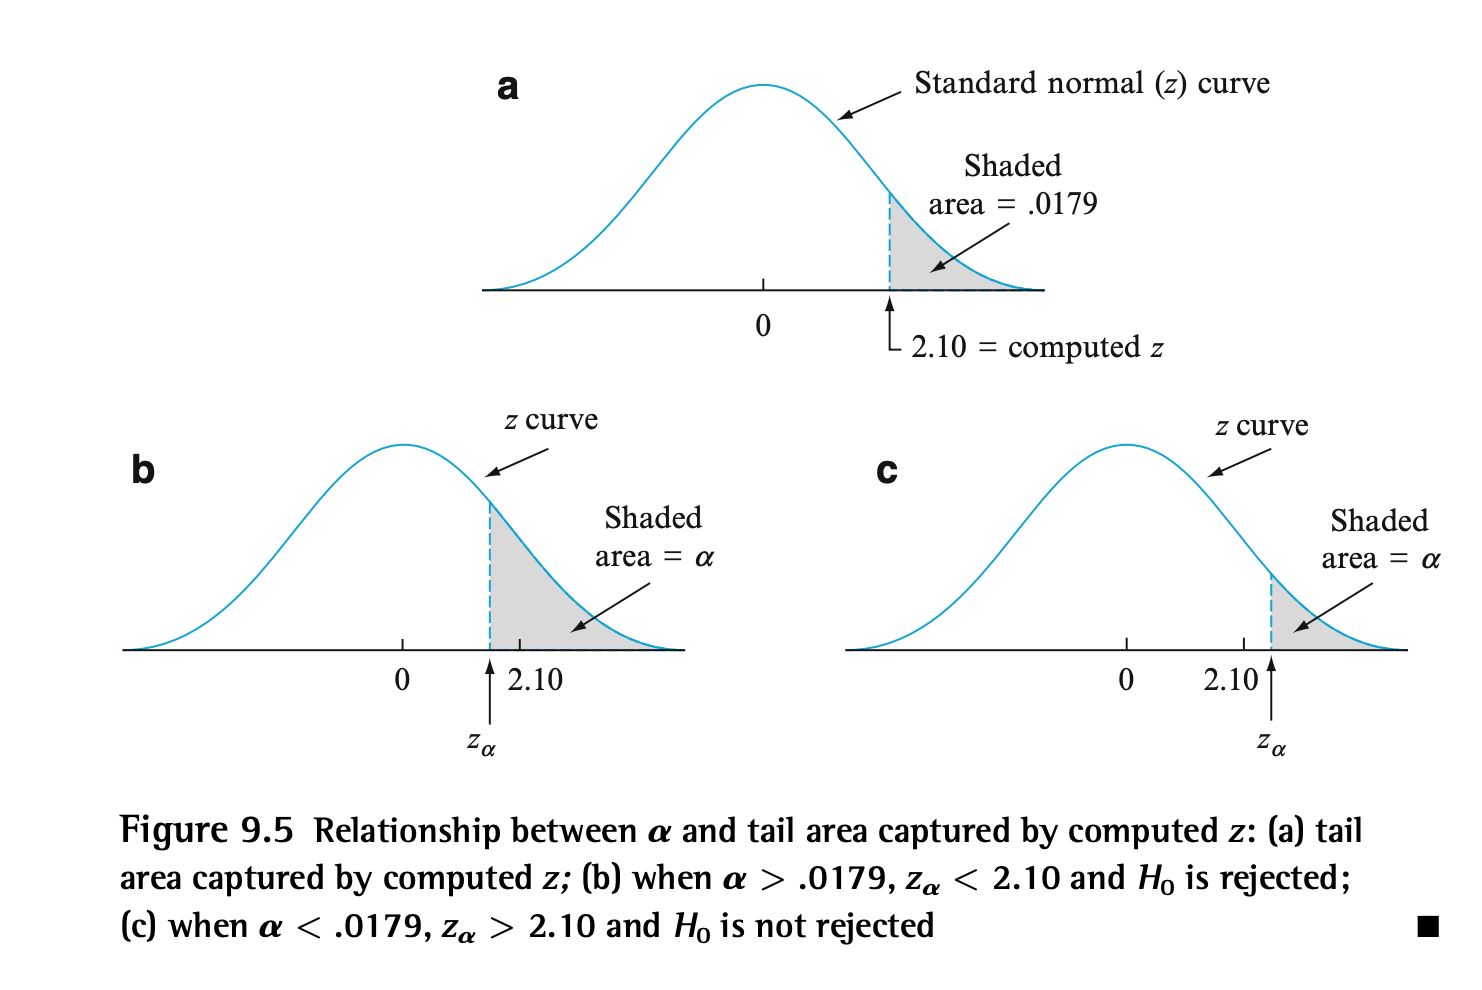
\includegraphics{images/p-value.png}
\end{frame}

\begin{frame}{P-value}
\protect\hypertarget{p-value-2}{}
\begin{tcolorbox}[enhanced jigsaw, left=2mm, breakable, bottomrule=.15mm, colframe=quarto-callout-important-color-frame, arc=.35mm, leftrule=.75mm, colbacktitle=quarto-callout-important-color!10!white, titlerule=0mm, opacityback=0, coltitle=black, opacitybacktitle=0.6, colback=white, toprule=.15mm, toptitle=1mm, bottomtitle=1mm, title=\textcolor{quarto-callout-important-color}{\faExclamation}\hspace{0.5em}{Proposition}, rightrule=.15mm]

The p-value is the smallest significance level \(\alpha\) at which the
null hypothesis can be rejected. Because of this, the p-value is
alternatively referred to as the \textbf{observed significance level
(OSL)} for the data.

\end{tcolorbox}

\begin{itemize}[<+->]
\tightlist
\item
  It is customary to call the data \emph{significant} when \(H_{0}\) is
  rejected and \emph{not significant} otherwise.
\end{itemize}
\end{frame}

\begin{frame}{Exercise 46}
\protect\hypertarget{exercise-46}{}
Pairs of p-values and significant levels, \(\alpha\), are given. For
each pair, state whether the observed p-value would lead to rejection of
\(H_{0}\) at the given significance level.

\begin{enumerate}[<+->]
[a.]
\tightlist
\item
  p-value = 0.084, \(\alpha = 0.05\)
\end{enumerate}

No! Fail to reject \(H_{0}\) since p-value \(\ngeq \alpha\).

\begin{enumerate}[<+->]
[a.]
\setcounter{enumi}{1}
\tightlist
\item
  p-value = 0.003, \(\alpha = 0.001\).
\end{enumerate}

No! Fail to reject \(H_{0}\) since p-value \(\ngeq \alpha\).
\end{frame}

\begin{frame}{Check in}
\protect\hypertarget{check-in}{}
Reject \(H_{0}\) true or false?

\begin{enumerate}[<+->]
[a.]
\setcounter{enumi}{2}
\item
  p-value = 0.498, \(\alpha\) = 0.05
\item
  p-value = 0.084, \(\alpha = 0.10\)
\item
  p-value = 0.039, \(\alpha = 0.10\).
\end{enumerate}
\end{frame}

\begin{frame}{P-value for z tests}
\protect\hypertarget{p-value-for-z-tests}{}
\begin{itemize}[<+->]
\tightlist
\item
  Consider an upper-tailed test and let \(z\) denote the computed value
  of the test statistic \(Z\).
\item
  The null hypothesis is rejected if \(z \geq z_{\alpha}\), and the
  p-value is the smallest \(\alpha\) for which this is the case.
\item
  Since \(z_{\alpha}\) increases as \(\alpha\) decreases, the p-value is
  the value of \(\alpha\) for which \(z = z_{\alpha}\)
\item
  That is, the p-value is just the area captured by the computed value
  \(z\) in the upper tail of the standard normal curve.
\item
  The corresponding cumulative area is \(\Phi(z)\), so in this case,
  p-value = \(1 - \Phi(z)\).
\end{itemize}
\end{frame}

\begin{frame}{P-values for z tests}
\protect\hypertarget{p-values-for-z-tests}{}
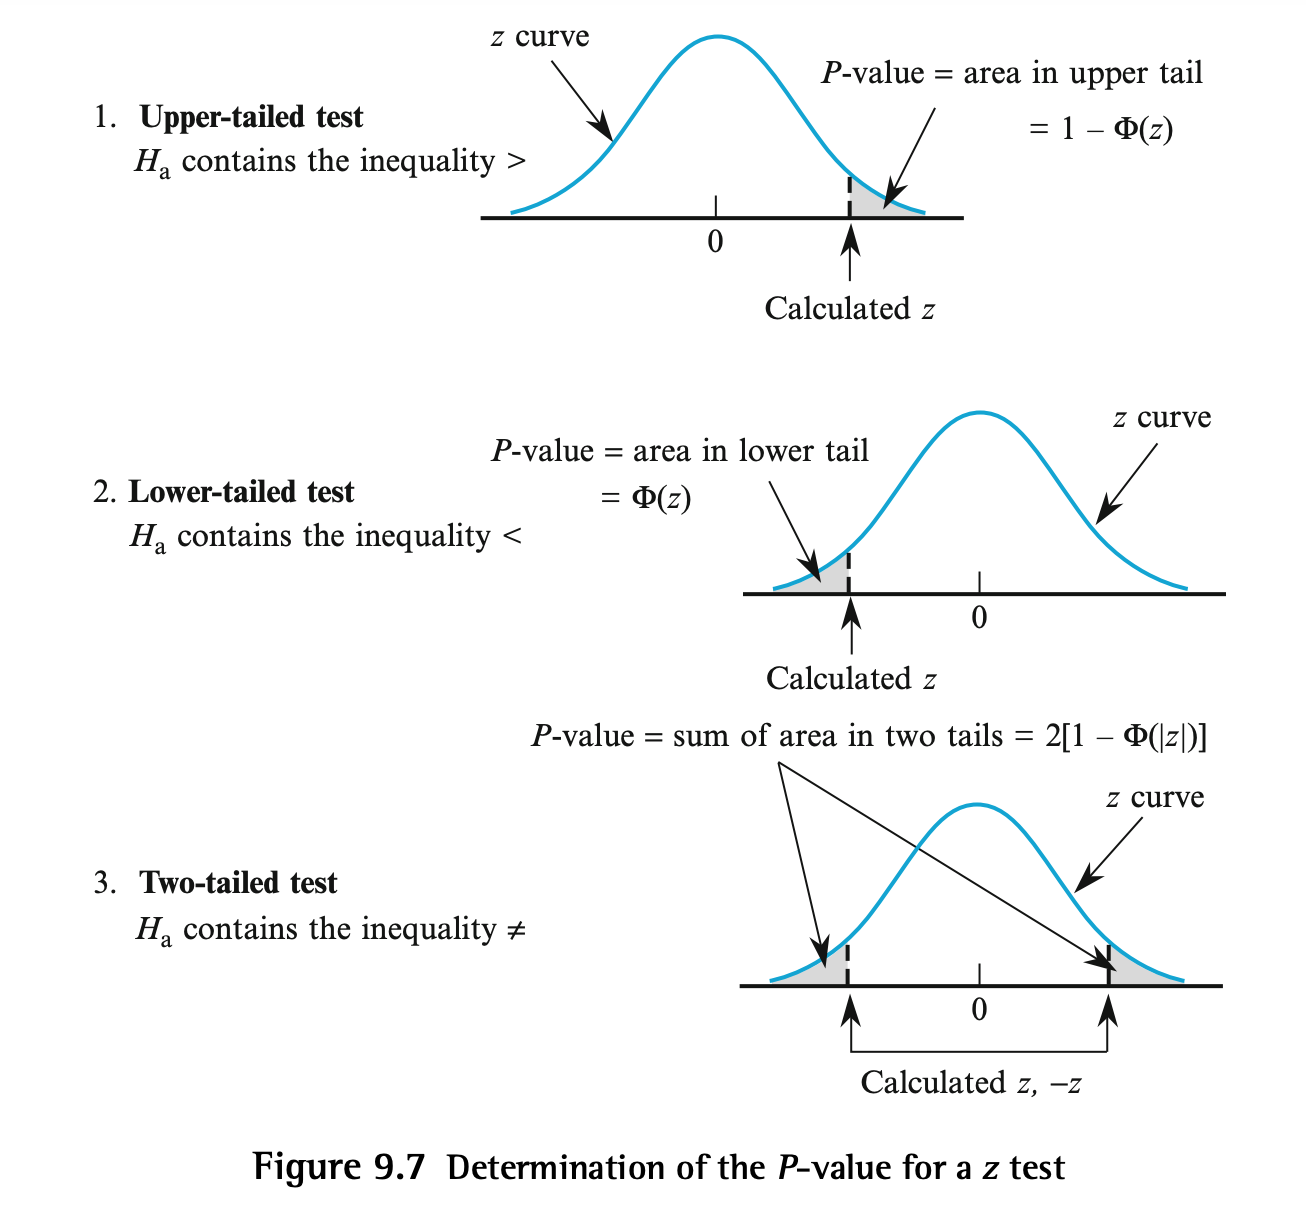
\includegraphics{images/pvaluecalc.png}
\end{frame}

\begin{frame}{P-values for z tests}
\protect\hypertarget{p-values-for-z-tests-1}{}
\begin{tcolorbox}[enhanced jigsaw, left=2mm, breakable, bottomrule=.15mm, colframe=quarto-callout-important-color-frame, arc=.35mm, leftrule=.75mm, colbacktitle=quarto-callout-important-color!10!white, titlerule=0mm, opacityback=0, coltitle=black, opacitybacktitle=0.6, colback=white, toprule=.15mm, toptitle=1mm, bottomtitle=1mm, title=\textcolor{quarto-callout-important-color}{\faExclamation}\hspace{0.5em}{P-values for Z tests}, rightrule=.15mm]

\[ 
\text{P-value}: \hspace{1cm} P = \begin{cases}
1-\Phi(z) & \text{ for an upper-tailed test} \\
\Phi(z) & \text{ for a lower-tailed test}\\
2[1 - \Phi(|z|)] & \text{ for a two-tailed test} 
\end{cases}
\]

\end{tcolorbox}
\end{frame}

\begin{frame}{Exercise 52}
\protect\hypertarget{exercise-52}{}
An aspirin manufacturer fills bottles by weight rather than by count.
Since each bottle should contain 100 tablets, the average weight per
tablet should be 5 grains. Each of 100 tablets taken from a very large
lot is weighed, resulting in a sample average weight per tablet of 4.87
grains and a sample standard deviation of 0.35 grain. Does this
information provide strong evidence for concluding that the company is
not filling its bottles as advertised? Test the appropriate hypothesis
using \(\alpha = 0.01\) by first computing the p-value and then
comparing it to the specified significance level.
\end{frame}

\begin{frame}{P-values for t Tests}
\protect\hypertarget{p-values-for-t-tests}{}
\begin{itemize}[<+->]
\tightlist
\item
  Just as the p-value for a z test is a z curve area, the p-value for a
  t test will be a t curve area.
\item
  Recall that the degrees of freedom for the one-sample t test is
  \(n-1\).
\item
  The table of t critical values used previously for confidence and
  prediction intervals doesn't contain enough information about any
  particular \(t\) distribution to allow for accurate determination of
  desired areas.
\item
  However, it is enough for us to get \textbf{bounds} on the p-value to
  make a decision.
\end{itemize}
\end{frame}

\begin{frame}{P-values for t tests}
\protect\hypertarget{p-values-for-t-tests-1}{}
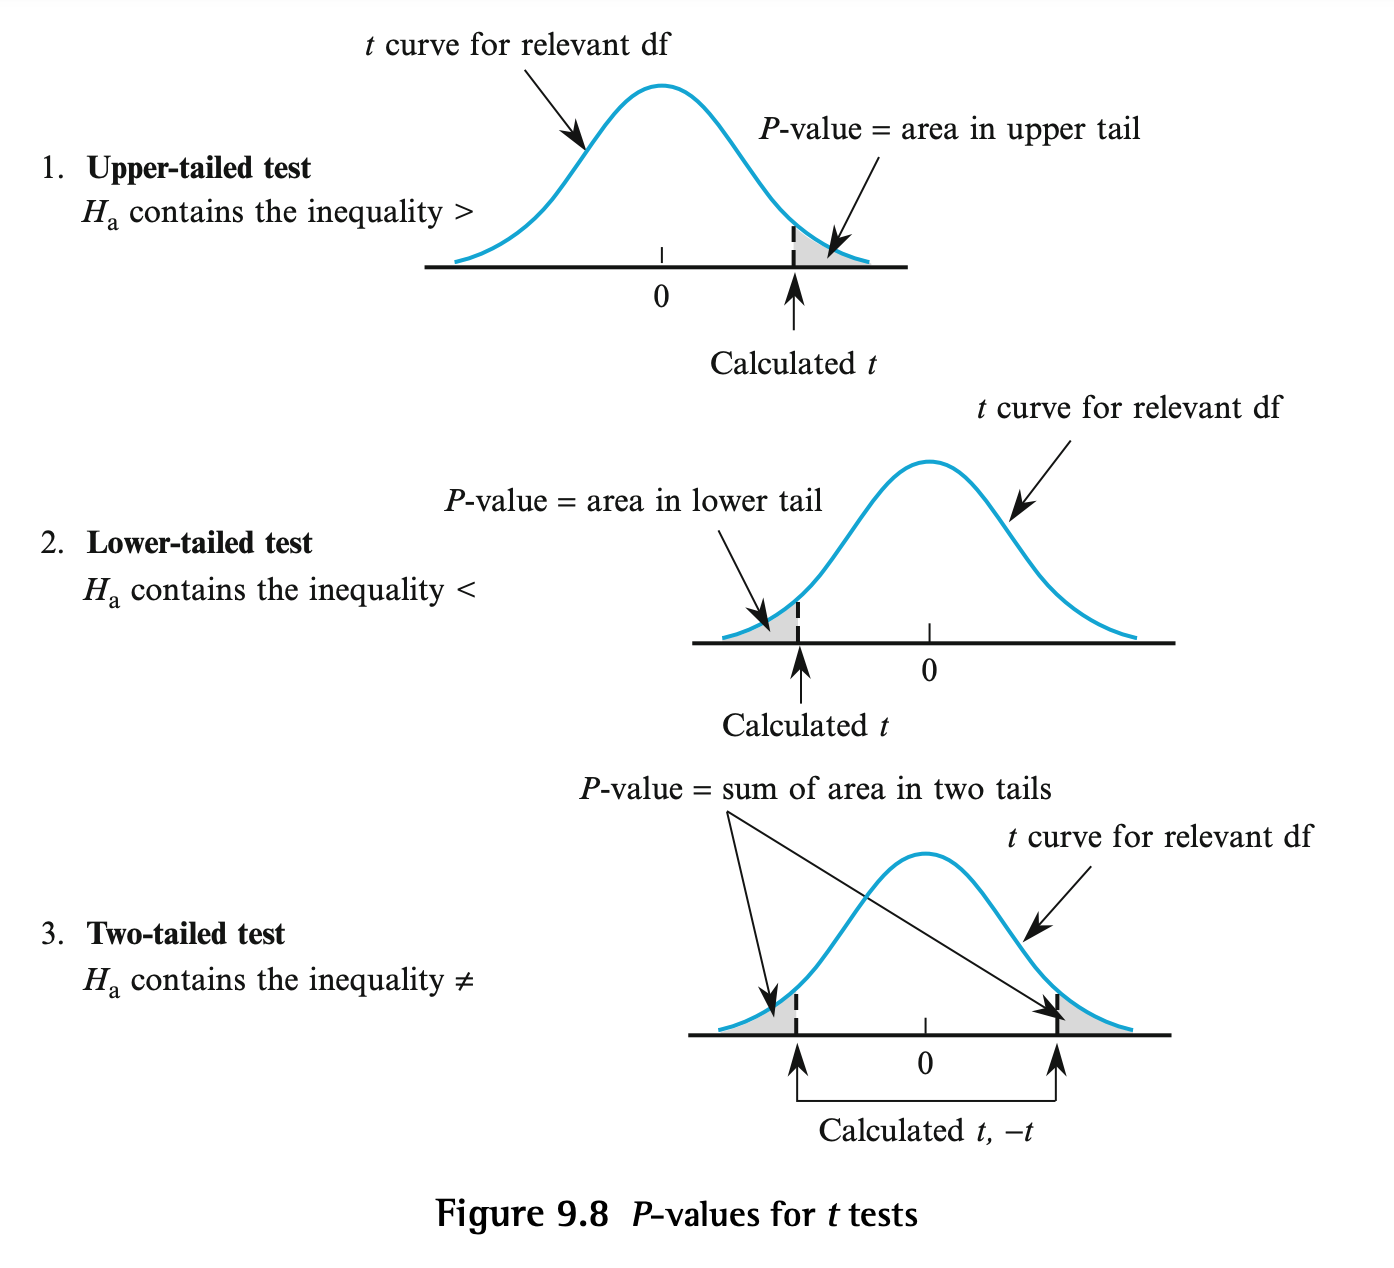
\includegraphics{images/pvaluetcalc.png}
\end{frame}

\begin{frame}{Exercise 58}
\protect\hypertarget{exercise-58}{}
A spectrophotometer used for measuring CO concentration {[}ppm (parts
per million) by volume{]} is checked for accuracy by taking readings on
a manufactured gas (called span gas) in which the CO concentration is
very precisely controlled at 70 ppm. If the readings suggest that the
spectrophotometer is not working properly, it will have to be
recalibrated. Assume that if it is properly calibrated, measured
concentration for span gas samples is normally distributed. On the basis
of the six readings---85, 77, 82, 68, 72, and 69---is recalibration
necessary? Carry out a test of the relevant hypotheses using the p-value
approach with \(\alpha = 0.05\). (\(\bar{x} = 75.5\), \(s = 7.0071\))
\end{frame}

\begin{frame}{Exercise 58 Solutions}
\protect\hypertarget{exercise-58-solutions}{}
\begin{enumerate}[<+->]
\tightlist
\item
  \(\mu\) = true average concentration reading of CO for span gas
  samples
\item
  \(H_{0}: \mu = 70\)
\item
  \(H_{a}: \mu \neq 70\)
\item
  \(T = \frac{\bar{X} - 70}{S/\sqrt{n}}\)
\item
  \(t = \frac{\bar{x} - 70}{s/\sqrt{n}} = \frac{75.5 - 70}{7.0071/\sqrt{6}} = 1.92\)\\
  \(df = n-1 = 5\)
\item
  pvalue =
  \(2P(T \geq 1.92) \rightarrow 2(0.05 < p-value < 0.10) \rightarrow 0.10 < pvalue < 0.20\).
\item
  \(\alpha = 0.05\), \(p-value > 0.10 > 0.05\), therefore, fail to
  reject \(H_{0}\) for \(H_{a}\). Therefore, at 5\% significance, we do
  not have enough evidence to say that the true average concentration
  reading of CO for span gas samples differs from 70ppm, so it does not
  need to be recalibrated.
\end{enumerate}
\end{frame}

\begin{frame}{Exercise 54}
\protect\hypertarget{exercise-54}{}
Many consumers are turning to generics as a way of reducing the cost of
prescription medications. The article ``Commercial Information on Drugs:
Confusing to the Physician?'' gives the results of a survey of 102
doctors. Only 47 of those surveyed knew the generic name for the drug
methadone. Does this provide strong evidence for concluding that fewer
than half of all physicians know the generic name for methadone? Carry
out a test of hypotheses with a significance level of \(0.01\) using the
p-value method.
\end{frame}

\begin{frame}{Summary}
\protect\hypertarget{summary-6}{}
\begin{itemize}[<+->]
\tightlist
\item
  The \textbf{p-value} is the probability, calculated assuming that the
  null hypothesis is true, of obtaining a value of the test statistic at
  least as contradictory to \(H_{0}\) as the value calculated from the
  available sample.
\item
  Reject \(H_{0}\) for \(H_{a}\) if p-value \(\leq \alpha\).
\item
  The p-value is the smallest significance level \(\alpha\) at which the
  null hypothesis can be rejected and is sometimes referred to as the
  \textbf{observed significance level (OSL)} for the data.
\end{itemize}
\end{frame}

\begin{frame}{Practice Problems}
\protect\hypertarget{practice-problems-3}{}
\begin{itemize}[<+->]
\tightlist
\item
  Odd problems 9.45 - 9.59
\end{itemize}
\end{frame}

\hypertarget{some-comments-on-selecting-a-test-procedure}{%
\section{9.5 Some Comments on Selecting a Test
Procedure}\label{some-comments-on-selecting-a-test-procedure}}

\begin{frame}{Outcomes}
\protect\hypertarget{outcomes-4}{}
By the end of this section, you will be able to:

\begin{itemize}[<+->]
\tightlist
\item
  Understand the difference between statistical and practical
  significance.
\item
  Know when to, and how to, apply the Neyman-Pearson Theorem.
\item
  Know what an UMP test is and how to find it.
\item
  Know what an unbiased test is.
\item
  Know how to find a likelihood ratio test.
\end{itemize}
\end{frame}

\begin{frame}{Comments}
\protect\hypertarget{comments}{}
\begin{itemize}[<+->]
\tightlist
\item
  Once the experimenter has decided on the question of interest and the
  method for gathering data (the design of the experiment), construction
  of an appropriate test procedure consists of three distinct steps:
\end{itemize}

\begin{enumerate}[<+->]
\tightlist
\item
  Specify a test statistic (the decision is based on this function of
  the data).
\item
  Decide on the general form of the rejection region (typically, reject
  \(H_{0}\) for suitably large values of the test statistic, reject for
  suitably small values, or reject for either small or large values).
\item
  Select the specific numerical critical value or values that will
  separate the rejection region from the non-rejection region (by
  obtaining the distribution of the test statistic when \(H_{0}\) is
  true, and then selecting a level of significance).
\end{enumerate}
\end{frame}

\begin{frame}{Comments}
\protect\hypertarget{comments-1}{}
This leads to some issues to be considered while carrying out these
steps. Specifically,

\begin{enumerate}[<+->]
\tightlist
\item
  What are the practical implications and consequences of choosing a
  particular level of significance once the other aspects of a test
  procedure have been determined?
\item
  Does there exist a general principle, not dependent just on intuition,
  that can be used to obtain best or good test procedures?
\item
  When two or more tests are appropriate in a given situation, how can
  the tests be compared to decide which should be used?
\item
  If a test is derived under specific assumptions about the distribution
  or population being sampled, how well will the test procedure work
  when the assumptions are violated?
\end{enumerate}
\end{frame}

\begin{frame}{Statistical Versus Practical Significance}
\protect\hypertarget{statistical-versus-practical-significance}{}
\begin{itemize}[<+->]
\tightlist
\item
  As we have learned, a small p-value indicates \textbf{statistical
  significance} in that it would strongly suggest rejection of \(H_{0}\)
  in favour of \(H_{a}\).
\item
  This, however, may be the result of a large sample size in combination
  with a departure from \(H_{0}\) that has little \textbf{practical
  significance}.
\item
  In many experimental situations, only departures from \(H_{0}\) of
  large magnitude would be worthy of detection, whereas a small
  departure from \(H_{0}\) would have little practical significance.
\end{itemize}
\end{frame}

\begin{frame}{Statistical Versus Practical Significance}
\protect\hypertarget{statistical-versus-practical-significance-1}{}
Example: A large insurance company mined its data and found a
statistically significant (p-value = 0.04) difference between the mean
value of policies sold in 2015 and 2016. The difference in the mean
values was \$9.83. Even though it was statistically significant,
management did not see this as an important difference when a typical
policy sold for more than \$1000.

On the other hand, even a clinically important improvement of 10\% in
the cure rate with a new treatment is not likely to produce
statistically significant results in a study of fewer than 225 patients.
A small clinic trial would probably not be conclusive.
\end{frame}

\begin{frame}{Practical Significance}
\protect\hypertarget{practical-significance}{}
\begin{itemize}[<+->]
\tightlist
\item
  For example, let \(\mu\) denote the true average IQ score in the very
  large city of Euphoria.
\item
  Consider testing \(H_{0}: \mu = 100\) versus \(H_{a}: \mu > 100\),
  assuming a normal IQ distribution with \(\sigma = 15\).
\item
  But one IQ point is no big deal, so the value \(\mu = 101\) certainly
  does not represent a departure from \(H_{0}\) that has practical
  significance.
\item
  The table on the next slide shows the relationship between the sample
  size and p-value and \(\beta\).
\end{itemize}
\end{frame}

\begin{frame}{Practical Significance}
\protect\hypertarget{practical-significance-1}{}
\begin{longtable}[]{@{}
  >{\raggedright\arraybackslash}p{(\columnwidth - 4\tabcolsep) * \real{0.1111}}
  >{\raggedright\arraybackslash}p{(\columnwidth - 4\tabcolsep) * \real{0.4167}}
  >{\raggedright\arraybackslash}p{(\columnwidth - 4\tabcolsep) * \real{0.4722}}@{}}
\toprule()
\begin{minipage}[b]{\linewidth}\raggedright
n
\end{minipage} & \begin{minipage}[b]{\linewidth}\raggedright
p-value when \(\bar{x} = 101\)
\end{minipage} & \begin{minipage}[b]{\linewidth}\raggedright
\(\beta(101)\) for level 0.01 test
\end{minipage} \\
\midrule()
\endhead
25 & 0.3707 & 0.9772 \\
100 & 0.2514 & 0.9525 \\
400 & 0.0918 & 0.8413 \\
900 & 0.0228 & 0.6293 \\
1600 & 0.0038 & 0.3707 \\
2500 & 0.0004 & 0.1587 \\
5000 & 0.0000012 & 0.0087 \\
10,000 & 0.0000000 & 0.0000075 \\
\bottomrule()
\end{longtable}
\end{frame}

\begin{frame}{Practical Significance}
\protect\hypertarget{practical-significance-2}{}
\begin{itemize}[<+->]
\tightlist
\item
  Even for moderately large ample sizes, the p-value resulting from
  \(\bar{x} = 101\) argues very strongly for the rejection of \(H_{0}\)
  for \(H_{a}\), whereas the observed \(\bar{x}\) itself suggests that
  in practical terms, the true value of \(\mu\) differs little from the
  null value of \(\mu_{0} = 100\).
\item
  The third column points out that even when there is little practical
  difference between \(\mu\) and the null value, for a fixed level of
  significance a large sample size will frequently lead to rejection of
  the null hypothesis at that level.
\item
  To summarize, one must be especially careful in interpreting evidence
  when the sample size is large, since any small departure from
  \(H_{0}\) will almost certainly be detected by a test, yet such a
  departure may have little practical significance.
\end{itemize}
\end{frame}

\begin{frame}{Example 60}
\protect\hypertarget{example-60}{}
Reconsider the pain-drying problem discussed in Example 9.2, The
hypotheses were \(H_{0}: \mu = 75\) versus \(H_{a}: \mu < 75\) with
\(\sigma\) assumed to have value 9.0. Consider the alternative value
\(\mu = 74\), which in the context of the problem would presumably not
be practically significant departure from \(H_{0}\).

\begin{enumerate}[<+->]
[a.]
\tightlist
\item
  For a level 0.01 test, compute \(\beta\) at this alternative for
  sample sizes \(n=100\), \(n=900\) and \(n=2500\).
\item
  If the observed value of \(\bar{X}\) is \(\bar{x} = 74\), what can you
  say about the resulting p-value when \(n=2500\)? Is the data
  statistically significant at any of the standard values of \(\alpha\)?
\item
  Would you really want to use a sample size of \(n=2500\) along with a
  level 0.01 test (disregarding the cost of such an experiment)?
  Explain.
\end{enumerate}
\end{frame}

\begin{frame}{Best Tests}
\protect\hypertarget{best-tests}{}
\begin{itemize}[<+->]
\tightlist
\item
  We've talked about a lot of tests, but haven't discussed whether they
  are the best way of testing the hypotheses.
\item
  That is, we ideally want \(\beta\) to be as small as possible while
  controlling \(\alpha\).
\item
  Let's first consider \textbf{simple hypotheses}, that is, hypotheses
  that completely specify the distribution of \(X_{i}\).
\item
  For example, it we know \(X_{i}\) follows an exponential distribution
  with parameter \(\lambda\), then \(H_{0}: \lambda = 1\) completely
  specifies the distribution. Similarly, \(H_{a}: \lambda = 2\)
  completely species the distribution. However, \(H_{a}: \lambda > 1\)
  does not completely specify the distribution since \(\lambda\) could
  be 2, or 5, or 300.
\end{itemize}
\end{frame}

\begin{frame}{Neyman-Pearson Theorem \{.smaller}
\protect\hypertarget{neyman-pearson-theorem-.smaller}{}
\begin{tcolorbox}[enhanced jigsaw, left=2mm, breakable, bottomrule=.15mm, colframe=quarto-callout-important-color-frame, arc=.35mm, leftrule=.75mm, colbacktitle=quarto-callout-important-color!10!white, titlerule=0mm, opacityback=0, coltitle=black, opacitybacktitle=0.6, colback=white, toprule=.15mm, toptitle=1mm, bottomtitle=1mm, title=\textcolor{quarto-callout-important-color}{\faExclamation}\hspace{0.5em}{Theorem}, rightrule=.15mm]

For testing a simple null hypotheses \(H_{0}: \theta = \theta_{0}\)
versus a simple alternative hypotheses \(H_{a}: \theta = \theta_{a}\),
let \(k\) be a positive fixed number and form the rejection region

\[ 
R^{*} = \left\{(x_{1},...,x_{n}): \frac{f(x_{1},...,x_{n};\theta_{a})}{f(x_{1},...,x_{n};\theta_{0})} \geq k \right\}
\]

Thus, \(R^{*}\) is the set of all observations for which the likelihood
ratio - the ratio of the alternative likelihood to the null likelihood -
is at least \(k\). The probability of a type I error for the test with
this rejection region is
\(\alpha^{*} = P[(X_{1},...,X_{n}) \in R^{*} \text{ when } \theta = \theta_{0}]\),
whereas the type II error probability \(\beta^{*}\) is the probability
that the \(X_{i}\)'s lie in the complement of \(R^{*}\) when
\(\theta = \theta_{a}\).

Then for any other test procedure with type I error probability
\(\alpha\) satisfying \(\alpha \leq \alpha^{*}\), the probability of a
type II error must satisfy \(\beta \geq \beta^{*}\). Thus the test with
rejection region \(R^{*}\) has the smallest type II error probability
among all tests for which the type I error probability is at most
\(\alpha^{*}\).

\end{tcolorbox}
\end{frame}

\begin{frame}{Example 9.20}
\protect\hypertarget{example-9.20}{}
Consider randomly selecting \(n=5\) new vehicles of a certain type and
determining the number of major defects on each one. Letting \(X_{i}\)
denote the number of such defects for the \(i^{th}\) selected vehicle
(i= 1,\ldots,5), suppose that the \(X_{i}\)'s form a random sample from
a Poisson distribution with parameter \(\lambda\). Let's find the best
test for testing \(H_{0}: \lambda = 1\) versus \(H_{a}: \lambda = 2\).
The poisson likelihood is

\[
f(x_{1},...,x_{5};\lambda = e^{-5\lambda}\lambda^{\sum x_{i}}/\Pi x_{i}!)
\]

Substituting first \(\lambda = 2\) then \(\lambda = 1\) and then taking
the ratio of these two likelihoods gives the rejection region:

\[
R^{*} = \{(x_{1},...,x_{5}):e^{-5}2^{\sum x_{i}} \geq k\}
\]
\end{frame}

\begin{frame}{Example 9.20}
\protect\hypertarget{example-9.20-1}{}
Multiplying both sides of the inequality by \(e^{5}\) and letting
\(k^{\prime} = ke^{5}\) gives the rejection region
\(2^{\sum x_{i}} \geq k^{\prime}\). Now take the natural logarithm of
both sides and let \(c = ln(k^{\prime})/ln(2)\) to obtain the rejection
region \(\sum x_{i} \geq c\).

This latter rejection region is completely equivalent to \(R^{*}\).
\(T = \sum X_{i}\) has a Poisson distribution with parameter
\(5\lambda\), so when \(H_{0}\) is true, T has a Poisson distribution
with parameter \(5\). From Table A.2, the cumulative probabilities for
the values 8 and 9 are 0.932 and 0.968, respectively. Thus, if we use
\(c = 9\) in the rejection region,

\[
\alpha^{*} = P(\text{Poisson rv with parameter 5 is } \geq 9) = 1 - 0.932 = 0.068
\]

Choosing instead \(c = 10\) gives \(\alpha^{*} = 0.032\). If we insist
that the significance level be at most 0.05, then the optimal rejection
region is \(\sum x_{i} \geq 10\).
\end{frame}

\begin{frame}{Example 9.20}
\protect\hypertarget{example-9.20-2}{}
When \(H_{a}\) is true, the test statistic has a Poisson distribution
with parameter 10. Thus

\[
\begin{aligned}
\beta^{*} &= P(H_{0} \text{ is not rejected when } H_{a} \text{ is true}) \\
&= P(\text{Poisson rv with parameter 10 is } \leq 9) \\
&= 0.458
\end{aligned}
\]
\end{frame}

\begin{frame}{Power and Uniformly Most Powerful Tests}
\protect\hypertarget{power-and-uniformly-most-powerful-tests}{}
\begin{itemize}[<+->]
\tightlist
\item
  The Neyman-Pearson theorem can be restated in a slightly different way
  by considering the \emph{power of a test}, \(1 - \beta\).
\end{itemize}

\begin{tcolorbox}[enhanced jigsaw, left=2mm, breakable, bottomrule=.15mm, colframe=quarto-callout-important-color-frame, arc=.35mm, leftrule=.75mm, colbacktitle=quarto-callout-important-color!10!white, titlerule=0mm, opacityback=0, coltitle=black, opacitybacktitle=0.6, colback=white, toprule=.15mm, toptitle=1mm, bottomtitle=1mm, title=\textcolor{quarto-callout-important-color}{\faExclamation}\hspace{0.5em}{Definition}, rightrule=.15mm]

Let \(\Omega_{0}\) and \(\Omega_{a}\) be two disjoint sets of possible
values of \(\theta\), and consider testing
\(H_{0}: \theta \in \Omega_{0}\) versus \(H_{a}: \theta \in \Omega_{a}\)
using a test with rejection region \(R\). Then the \textbf{power
function} of the test, denoted by \(\pi(\cdot)\) is the probability of
rejecting \(H_{0}\) considered as a function of \(\theta\):

\[ 
\pi(\theta^{\prime}) = P[(X_{1},...,X_{n}) \in R \text{ when } \theta = \theta^{\prime}]
\]

\end{tcolorbox}

\begin{itemize}[<+->]
\tightlist
\item
  Since we don't want to reject the null hypothesis when
  \(\theta \in \Omega_{0}\) and do want to reject it when
  \(\theta \in \Omega_{a}\), we wish a test for the which the power
  function is close to 0 whenever \(\theta^{\prime}\) is in
  \(\Omega_{0}\) and close to 1 whenever \(\theta^{\prime}\) is in
  \(\Omega_{a}\).
\end{itemize}
\end{frame}

\begin{frame}{Power and Uniformly Most Powerful Tests}
\protect\hypertarget{power-and-uniformly-most-powerful-tests-1}{}
\begin{itemize}[<+->]
\tightlist
\item
  The power is easily related to the type I and type II error
  probabilities:
\end{itemize}

\[
\pi(\theta^{\prime}) = \begin{cases}
P(\text{type I error when }\theta = \theta^{\prime}) = \alpha(\theta^{\prime}) & \text{ when } \theta^{\prime} \in \Omega^{0} \\
1 - P(\text{type II error when }\theta = \theta^{\prime}) = 1 - \beta(\theta^{\prime}) & \text{ when } \theta^{\prime} \in \Omega^{a}
\end{cases}
\]
\end{frame}

\begin{frame}{Example 62}
\protect\hypertarget{example-62}{}
For a random sample of \(n\) individuals taking a licensing exam, let
\(X_{i} = 1\) if the \(i^{th}\) individual in the sample passes, and
\(X_{i} = 0\) otherwise.

\begin{enumerate}[<+->]
[a.]
\tightlist
\item
  With \(p\) denoting the proportion of all exam takers who pass, show
  that the most powerful test of \(H_{0}: p = 0.5\) versus
  \(H_{a}: p = 0.75\) rejects \(H_{0}\) when \(\sum x_{i} \geq c\).
\item
  If \(n=20\) and you want \(\alpha \leq 0.05\) for the test of (a),
  would you reject \(H_{0}\) if 15 of the 20 individuals in the sample
  pass the exam?
\item
  What is the power of the test you used in (b) when \(p=0.75\).
\end{enumerate}
\end{frame}

\begin{frame}{Uniformly Most Powerful Tests}
\protect\hypertarget{uniformly-most-powerful-tests}{}
\begin{tcolorbox}[enhanced jigsaw, left=2mm, breakable, bottomrule=.15mm, colframe=quarto-callout-important-color-frame, arc=.35mm, leftrule=.75mm, colbacktitle=quarto-callout-important-color!10!white, titlerule=0mm, opacityback=0, coltitle=black, opacitybacktitle=0.6, colback=white, toprule=.15mm, toptitle=1mm, bottomtitle=1mm, title=\textcolor{quarto-callout-important-color}{\faExclamation}\hspace{0.5em}{Definition}, rightrule=.15mm]

A \textbf{uniformly most powerful (UMP) level} \(\alpha\) test is one
for which \(\pi(\theta^{\prime})\) is maximized for any
\(\theta \in \Omega_{a}\) subject to
\(\pi(\theta^{\prime}) \leq \alpha\) for any
\(\theta^{\prime} \in \Omega_{0}\).

Note: These are quite rare!

\end{tcolorbox}
\end{frame}

\begin{frame}{Unbiased Tests}
\protect\hypertarget{unbiased-tests}{}
\begin{tcolorbox}[enhanced jigsaw, left=2mm, breakable, bottomrule=.15mm, colframe=quarto-callout-important-color-frame, arc=.35mm, leftrule=.75mm, colbacktitle=quarto-callout-important-color!10!white, titlerule=0mm, opacityback=0, coltitle=black, opacitybacktitle=0.6, colback=white, toprule=.15mm, toptitle=1mm, bottomtitle=1mm, title=\textcolor{quarto-callout-important-color}{\faExclamation}\hspace{0.5em}{Definition}, rightrule=.15mm]

An \textbf{unbiased test} is a test for which the smallest value of
\(\pi(\theta^{\prime})\) for \(\theta^{\prime} \in \Omega_{a}\) is at
least as large as the largest value of \(\pi(\theta^{\prime})\) for
\(\theta^{\prime} \in \Omega_{0}\). This says that we are at least as
likely to reject the null hypothesis when \(H_{0}\) is false as we are
to reject it when \(H_{0}\) is true.

\end{tcolorbox}

\begin{itemize}[<+->]
\tightlist
\item
  It can be shown that the one-sample t test is UMP unbiased, that is,
  it is uniformly most powerful among all tests that are unbiased.
\end{itemize}
\end{frame}

\begin{frame}{Exercise 62}
\protect\hypertarget{exercise-62}{}
\begin{enumerate}[<+->]
[a.]
\setcounter{enumi}{3}
\tightlist
\item
  Is the test derived in (a) UMP for testing the hypotheses
  \(H_{0}: p = 0.5\) versus \(H_{a}: p > 0.5\)? Explain your reasoning.
\end{enumerate}
\end{frame}

\begin{frame}{Likelihood Ratio Tests}
\protect\hypertarget{likelihood-ratio-tests}{}
\begin{itemize}[<+->]
\tightlist
\item
  Mostly commonly used method for finding an appropriate test statistic
  in a new situation.
\item
  Recall, the joint pmf or pdf of \(X_{1}\),\ldots,\(X_{n}\) is denoted
  by \(f(x_{1},...,x_{n};\theta)\), which in the case of a random sample
  works out to be the product \(f(x_{1};\theta)\cdots f(x_{n};\theta)\).
\item
  When the \(x_{i}\)'s are the actual observations and
  \(f(x_{1},...,x_{n};\theta)\) is regarded as a function of \(\theta\),
  then it is called the likelihood function.
\item
  Consider testing \(H_{0}:\theta \in \Omega_{0}\) versus
  \(H_{a}: \theta \in \Omega_{a}\), where \(\Omega_{0}\) and
  \(\Omega_{a}\) are disjoint sets, and let
  \(\Omega = \Omega_{0} \cup \Omega_{a}\).
\end{itemize}
\end{frame}

\begin{frame}{Likelihood Ratio Tests}
\protect\hypertarget{likelihood-ratio-tests-1}{}
\begin{enumerate}[<+->]
\tightlist
\item
  Find the largest value of the likelihood for any
  \(\theta \in \Omega_{0}\) by finding the maximum likelihood testing of
  \(\theta\) within \(\Omega_{0}\) and substituting this mle into the
  likelihood function to obtain \(L(\hat\Omega_{0})\).
\item
  Find the largest value of the likelihood for any \(\theta \in \Omega\)
  by finding the maximum likelihood estimate of \(\theta\) within
  \(\Omega\) and substituting this mle into the likelihood function to
  obtain \(L(\hat\Omega)\). Because \(\theta_{0}\) is a subset of
  \(\Omega\), this likelihood \(L(\hat\Omega)\) can't be any smaller
  than the likelihood \(L(\hat\Omega_{0})\) obtained in the first step
  and will be much larger when the data is much more consistent with
  \(H_{a}\) than with \(H_{0}\).
\item
  Form the \emph{likelihood ratio} \(L(\hat{\Omega_{0}})/L(\hat\Omega)\)
  and reject the null hypothesis in favour of the alternative when this
  ratio is \(\leq k\). The critical value \(k\) is chosen to give a test
  with the desired significance level. In practice, the inequality
  \(L(\hat{\Omega_{0}})/L(\hat\Omega) \leq k\) is often re-expressed in
  terms of a more convenient statistic (such as the sum of the
  observations) whose distribution is known or can be derived.
\end{enumerate}
\end{frame}

\begin{frame}{Exercise 68}
\protect\hypertarget{exercise-68}{}
The error in a measurement is normally distributed with mean \(\mu\) and
standard deviation 1. Consider a random sample of \(n\) errors, and show
that the likelihood ratio test for \(H_{0}: \mu = 0\) versus
\(H_{a}: \mu \neq 0\) rejects the null hypothesis when either
\(\bar{x} \geq c\) or \(\bar{x} \leq -c\). What is \(c\) for a test with
\(\alpha = 0.05\)? How does the test change if the standard deviation is
\(\sigma_{0}\) (known) and the relevant hypotheses are
\(H_{0}: \mu = 0\) versus \(H_{a}: \mu \neq mu_{0}\).
\end{frame}

\begin{frame}{Summary}
\protect\hypertarget{summary-7}{}
\begin{itemize}[<+->]
\tightlist
\item
  Statistical significance occurs when the test results in a small
  p-value, however this may have no practical significance, which means
  that in reality, the difference does not serve any practical use (for
  example differences of a few cents or dollars).
\item
  The Neyman-Pearson Theorem says that for testing a simple null
  hypotheses \(H_{0}: \theta = \theta_{0}\) versus a simple alternative
  hypotheses \(H_{a}: \theta = \theta_{a}\), let \(k\) be a positive
  fixed number and form the rejection region
\end{itemize}

\[ 
R^{*} = \left\{(x_{1},...,x_{n}): \frac{f(x_{1},...,x_{n};\theta_{a})}{f(x_{1},...,x_{n};\theta_{0})} \geq k \right\}
\]

, then the test with rejection region \(R^{*}\) has the smallest
probability of type II error for any test with probability of type I
error at most \(\alpha\).
\end{frame}

\begin{frame}{Summary}
\protect\hypertarget{summary-8}{}
\begin{itemize}[<+->]
\tightlist
\item
  A \textbf{uniformly most powerful (UMP) level} \(\alpha\) test is one
  for which \(pi(\theta^{\prime})\) is maximized for any
  \(\theta \in \Omega_{a}\) subject to
  \(\pi(\theta^{\prime}) \leq \alpha\) for any
  \(\theta^{\prime} \in \Omega_{0}\).
\item
  An \textbf{unbiased test} is a test for which the smallest value of
  \(\pi(\theta^{\prime})\) for \(\theta^{\prime} \in \Omega_{a}\) is at
  least as large as the largest value of \(\pi(\theta^{\prime})\) for
  \(\theta^{\prime} \in \Omega_{0}\). This says that we are at least as
  likely to reject the null hypothesis when \(H_{0}\) is false as we are
  to reject it when \(H_{0}\) is true.
\item
  Form the \emph{likelihood ratio} \(L(\hat{\Omega_{0}})/L(\hat\Omega)\)
  and reject the null hypothesis in favour of the alternative when this
  ratio is \(\leq k\). The critical value \(k\) is chosen to give a test
  with the desired significance level.
\end{itemize}
\end{frame}

\begin{frame}{Practice Problems}
\protect\hypertarget{practice-problems-4}{}
\begin{itemize}[<+->]
\tightlist
\item
  Odd problems 61-69
\end{itemize}
\end{frame}



\end{document}
